% EMNLP 2026 long paper (8 pages + unlimited refs/appendix)
% AdapterFrontier
% Compile: pdflatex emnlp.tex; bibtex emnlp; pdflatex emnlp.tex; pdflatex emnlp.tex
% Uses official ACL style (acl.sty + acl_natbib.bst from acl-org/acl-style-files).

\documentclass[11pt]{article}
\usepackage[review]{acl}

\usepackage[T1]{fontenc}
\usepackage[utf8]{inputenc}
\usepackage{microtype}
\usepackage{inconsolata}
\usepackage{times}
\usepackage{booktabs}
\usepackage{graphicx}
\usepackage{placeins}
\usepackage{amsmath,amssymb}
\usepackage{url}
\usepackage{enumitem}

\title{What Adapter Ensembling Actually Buys:\\A Pre-Registered Audit, and the Scalar That Replaces the Population}

\author{
  Anonymous Authors \\
  Anonymous Affiliation \\
  \texttt{anonymous@example.org}
}

\date{}

\begin{document}
\maketitle

\begin{abstract}
Parameter-efficient fine-tuning leaves practitioners with populations of adapters, and a large literature reports that combining them helps. We ask what combining them actually buys once the single-adapter baseline is made strong. We pre-register and release \textsc{AdapterFrontier}, a $1{,}028$-cell corpus registered at git SHA \texttt{02a5a6bc} \emph{before any adapter was trained} ($67$ pools, $10$ architectures, $8$ tasks)\footnote{Cell count: $1{,}028 = 827$ v1.0 main-pool cells (55 pools $\times$ ensemble methods $\times$ \{\texttt{best\_of\_n}, \texttt{n\_rank}\} $\times$ \{accuracy, ECE\}) $+$ $100$ v1.1 HellaSwag multichoice cells $+$ $101$ baseline self-comparison cells. The $2$ v1.1 GSM8K and $7$ v1.2 supplementary pools (App.~\ref{app:prereg}) are reported separately in Table~\ref{tab:v11cells} and are not in the headline $1{,}028$.}, adjudicating every (pool, method, baseline, metric) cell with paired bootstrap CIs and corpus-wide BH-FDR control. Our single-adapter baseline is deliberately strong: measured from the released manifests it received a median $1.45\times$ the pool's training compute (and up to $2.96\times$) plus a hyperparameter search the ensemble arm never gets. Against that baseline, encoder ensembling \textbf{never significantly improves accuracy} --- $0$ of $92$ clean cells, identically before and after FDR correction, with $33.7\%$ significantly \emph{worse}. It does improve ECE on $52$ of the same $92$ cells, and we initially read that as a dissociation. It is not one. The comparison is against a single adapter chosen by validation \emph{accuracy} and never calibrated, which is the weak-baseline shortcut this paper is otherwise about; on the pools where we can run the missing control, \textbf{one temperature fitted on held-out data erases the advantage} (ensemble better in $4/6$ pools $\to$ $2/6$, mean $\Delta$ECE $-0.032$), the multiclass Brier never corroborated it ($34/92$), and the mechanism is confidence shrinkage --- which a scalar reproduces at $1\times$ inference cost. The practical consequence is to calibrate one adapter rather than serve $N$. We then quantify three evaluation shortcuts that each restore an apparent accuracy benefit: selecting the single adapter on test ($+1.12$pp on average), comparing against a same-size rather than a stronger single ($27.2\%$ vs.\ $9.9\%$ of cells SUPPORTED), and reporting task means (one $-0.012$pp ``no effect'' average conceals $37$ significant cells). We release the cells, per-example predictions, split manifests and adjudication code so new methods can be compared without retraining.
\end{abstract}

\section{Introduction}

Parameter-efficient fine-tuning (PEFT) with LoRA-style adapters \citep{hu2021lora} has made it routine to keep dozens of task-specific adapters around: serving stacks such as vLLM and S-LoRA \citep{kwon2023efficient,sheng2024slora} route per request to one of $N$ adapters at negligible extra cost, and frameworks such as LoRAHub \citep{huang2023lorahub} target multi-adapter composition directly. The practitioner's question is whether \emph{combining} those adapters --- averaging weights, voting on labels, or routing through them --- beats spending the same budget on a single adapter. A large literature reports that it does. We ask a prior question: \emph{how much of that reported benefit survives a strict evaluation protocol?}

Answering this requires comparisons that were fixed before the data was seen, because the choices involved --- which single adapter counts as the baseline, how it was selected, at what budget, and on which benchmark --- are exactly the choices that determine the answer. We therefore pre-registered \textsc{AdapterFrontier} at git SHA \texttt{02a5a6bc} \emph{before any adapter was trained}, and adjudicate each (pool, method, baseline, metric) cell independently with paired bootstrap CIs, sign-flip tests, and corpus-wide Benjamini--Hochberg FDR \citep{bh1995}.

\paragraph{A strong baseline, and a dissociation.} The comparison that decides this question is the single adapter you would train instead. We make that competitor deliberately strong: our pre-registered \texttt{n\_rank} baseline spends the pool's budget on adapter rank, and measured from the released manifests it in fact received a median $1.45\times$ the pool's training wall-clock (max $2.96\times$; $47$ of $48$ pool--baseline pairs favour the baseline) together with a rank$\times$epoch$\times$seed search selected on held-out data that the ensemble arm never receives. It also serves at $1\times$ inference cost against the ensemble's $N\times$. It is therefore a \emph{strict upper-bound} competitor rather than a matched one, which makes our accuracy null conservative. Against it, on the clean encoder slice: \textbf{no cell shows a significant accuracy gain} ($0$ of $92$, identically pre- and post-FDR) while $33.7\%$ are significantly reversed (mean $\Delta{=}{-}1.27$pp). Our pre-registration declared accuracy and calibration co-equal arms, and on \emph{the same $92$ cells} ensembling improves ECE in $52$. We read that as a dissociation until we noticed the comparison was not fair the way the accuracy arm's was: that single adapter is chosen by validation \emph{accuracy} and never calibrated. One temperature fitted on held-out data takes the ensemble from better-calibrated in $4/6$ pools to $2/6$ (\S\ref{sec:findings}). The honest statement is narrower and more useful: at fixed budget, populations buy neither accuracy nor reliability that a scalar cannot, at $1\times$ inference instead of $N\times$.

\paragraph{Three shortcuts restore the benefit.} That null result coexists with a literature reporting gains, so we measure what closes the gap (\S\ref{sec:protocol}). Selecting the ``best single'' on the test split is worth $+1.12$pp on average and inflates $82\%$ of pools. Comparing against a same-size single rather than a compute-matched one moves the SUPPORTED rate from $9.9\%$ to $27.2\%$. Reporting one mean per task hides the structure entirely: MNLI's $-0.012$pp average reads as ``no effect'' while concealing $37$ significant cells pointing in both directions. Each shortcut is individually defensible-looking; together they are enough to flip the sign of the conclusion.

\paragraph{Contributions.}
\textbf{(i)~A pre-registered corpus and adjudication framework}: $67$ adapter pools and $1{,}028$ cell JSONs with per-cell CIs, $p$-values and FDR-corrected verdicts, plus the locked pre-registration and amendment ledger; new methods are compared by submitting per-example predictions, with no retraining.
\textbf{(ii)~A null under a strong baseline, and the control that explains the one apparent exception}: against a single adapter that received more training compute and a hyperparameter search, PEFT ensembling never significantly improves encoder accuracy ($0/92$) and frequently harms it. It does improve ECE on $52$ of the same cells, but that comparison omits post-hoc calibration; supplying it removes most of the effect, which we trace to confidence shrinkage and replace with a single scalar.
\textbf{(iii)~A protocol-sensitivity analysis} quantifying three shortcuts that each restore an apparent benefit (Table~\ref{tab:protocol}, Fig.~\ref{fig:protocol}).
\textbf{(iv)~Negative results reported as such}: the diversity--quality frontier predicts accuracy deltas out of pool (corpus-wide LOPO-CV $R^2{=}0.597$ over $48$ pools, $95\%$ CI $[{+}0.30,{+}0.71]$; encoder-only $R^2{=}0.616$ over $23$ pools) but --- because those deltas are predominantly negative --- it predicts how much a pool stands to \emph{lose}; it does not extend to calibration, and three candidate mechanisms are tested and refuted (App.~\ref{app:mech}).

\paragraph{Descriptive regularities (oracle, not policy).}\label{sec:intro-rules} Cells do differ, and the differences are legible as five rules D1--D5 (App.~\ref{app:rules}). They were distilled from the same corpus they describe and evaluated on it, so they are an \emph{oracle upper bound}, not a deployable policy (L11) --- a prospective, validation-only version degenerated to always choosing the single adapter.

\begin{figure*}[t]
\centering
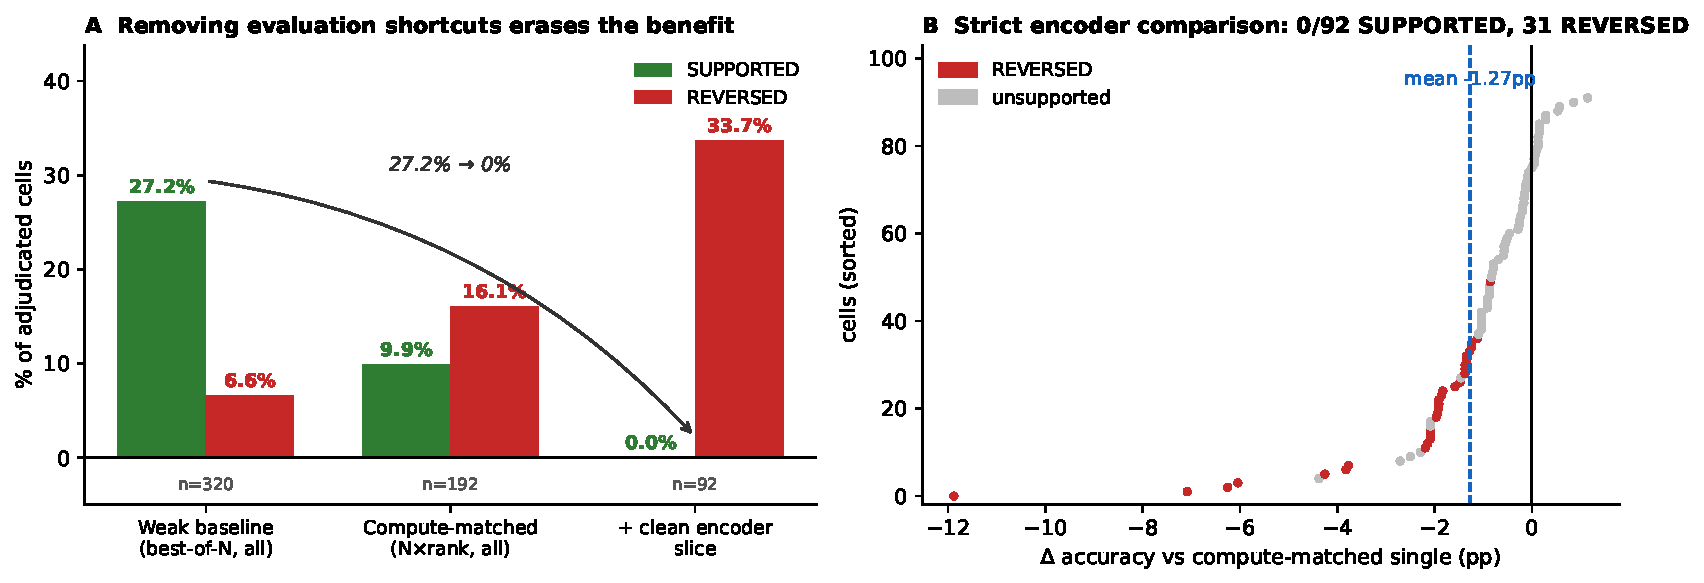
\includegraphics[width=\textwidth]{figures/fig1_protocol_sensitivity.pdf}
\caption{\textbf{The apparent ensembling benefit is a product of evaluation protocol.} \textbf{(A)} The fraction of cells adjudicated SUPPORTED collapses as shortcuts are removed: against the pool's own best single (\texttt{best\_of\_n}) $27.2\%$ of cells are SUPPORTED, against the pre-registered compute-matched single (\texttt{n\_rank}) $9.9\%$, and on the clean encoder slice \emph{none} are. REVERSED moves the other way ($6.6\%\!\to\!16.1\%\!\to\!33.7\%$). \textbf{(B)} All $92$ strict encoder cells, sorted, colored by post-FDR verdict: the mass lies left of zero (mean $-1.27$pp) and no cell is SUPPORTED.}
\label{fig:protocol}
\end{figure*}

\section{Related work}
\label{sec:related}

\paragraph{PEFT and adapter ensembling.} The adapter line of work begins with bottleneck adapters \citep{houlsby2019parameter} and the AdapterHub framework \citep{pfeiffer2020adapterhub}; LoRA \citep{hu2021lora}, DoRA \citep{dora}, PiSSA \citep{pissa}, AdaLoRA \citep{adalora}, and VeRA \citep{vera} make many low-rank adapters per task practical. Combination strategies split into three families: \emph{prediction-space} (soft/hard voting, logit averaging \citep{lakshminarayanan2017simple}); \emph{weight-space} (model soups \citep{wortsman2022model}, TIES \citep{yadav2023ties}, DARE \citep{yu2024dare}); and \emph{routing / mixture-of-adapters} (AdapterFusion \citep{pfeiffer2021adapterfusion} composes via attention; LoRAHub \citep{huang2023lorahub} optimizes a continuous weight vector; AdaMix \citep{adamix} mixes multiple LoRA experts inside training; MoLE \citep{mole} and MoLoRA \citep{molora} learn routing over adapter experts; HydraLoRA \citep{hydralora} uses asymmetric multi-head LoRA; MultiLoRA \citep{multilora} reduces interference among co-trained LoRAs). Our adjudication framework treats each of these methods as a \emph{plug-in} that produces per-example test predictions and can be added to our cell corpus without retraining the pools. We implement and report prediction-space methods directly (\texttt{soft\_vote}, \texttt{logit\_avg}, \texttt{majority\_vote}, \texttt{greedy\_soup}, plus a prediction-space \texttt{uniform\_soup} \emph{proxy} that averages per-adapter logits); weight-space TIES/DARE/uniform-merge implementations live in \texttt{weight\_space\_merge.py} and are reported as a separate family in App.~\ref{app:repro}. The cell JSONs include the input schema needed to evaluate routing/MoE methods (per-pool logits cache).


\paragraph{Pre-registration in ML.} Pre-registration is standard in clinical trials and increasingly common in cognitive science but rare in ML \citep{munafo2017manifesto, loken2017measurement}; \citet{hofman2021integrating} argue for tighter coupling of explanation and prediction in computational social science, an argument that translates directly to empirical NLP --- \citet{bowman2021will} make a closely related case that NLU benchmark results need pre-committed protocols if they are to drive scientific (rather than leaderboard) progress. \citet{dehghani2022efficiency} further argue that compute-matched comparisons are essential to honest efficiency claims --- a principle we apply across every cell. We adopt pre-registration here: the protocol, splits, baselines, and statistical tests were locked at git SHA \texttt{02a5a6bc} before any pool was trained.

\paragraph{Calibration of fine-tuned LMs.} ECE in its modern form was introduced by \citet{naeini2015}; the equal-mass 15-bin histogram became standard via \citet{guo2017calibration}, with refinements such as soft calibration objectives \citep{karandikar2021soft}. \citet{nixon2019} survey ECE estimator bias under varying bin counts and small-$N$ regimes; \citet{minderer2021} re-examine calibration of modern (post-2020) architectures and find that distribution-shift calibration does not always follow in-distribution calibration. Deep ensembles \citep{lakshminarayanan2017simple} reliably lower ECE on classifiers. We extend this measurement to PEFT pools and report Brier, NLL, MCE alongside ECE, with paired bootstrap CIs; per-token logprob ECE for generative tasks (App~\ref{app:stats}) is a non-standard adaptation we explicitly document.

\paragraph{Efficient multi-adapter serving.} S-LoRA \citep{sheng2024slora} and Punica \citep{chen2024punica} (the latter integrated in vLLM \citep{kwon2023efficient}) enable thousands of LoRA adapters to share a single base-model forward; we measure the runtime cost of cell-by-cell ensembling under this serving regime.

\paragraph{When reported gains do not survive fair comparison.} Several fields have found that a literature of reported improvements shrinks or disappears once baselines are tuned and budgets are matched: GAN variants become indistinguishable under equal hyperparameter search \citep{lucic2018gans}, deep metric-learning gains are ``marginal at best'' under controlled evaluation \citep{musgrave2020metric}, and most neural recommenders are beaten by simple heuristics \citep{dacrema2019progress}. The recurring cause is not fraud but protocol: an under-tuned or under-resourced baseline, a selection step that sees the test set, or an aggregate score that hides variance \citep{dodge2019show, reimers2017reporting}. NLP has documented the same failure modes for benchmarking practice \citep{bowman2021will} and for efficiency claims specifically, where comparisons that do not fix the compute budget can invert conclusions \citep{dehghani2022efficiency}. Two literatures bear directly on our question. PEFT evaluation has already had its reality check: \citet{chen2022revisiting} find validation and testing practice across PEFT studies unreliable once method instability is accounted for. And \emph{ensemble versus one bigger model at matched cost} is an open dispute rather than a naive assumption: \citet{abe2022deep} find a single larger network replicates ensemble gains with diversity contributing little, \citet{kondratyuk2020ensembling} conclude the opposite at matched FLOPs, \citet{lobacheva2020power} show the optimum depends on budget, and \citet{theisen2023ensembles} predict the gain from the disagreement-to-error ratio. Our accuracy result is the PEFT instance of the \citeauthor{abe2022deep} side; our frontier is consistent with \citeauthor{theisen2023ensembles}. We claim priority for neither. Ours is the pre-registration before training, the cell-level adjudication, the accuracy/calibration dissociation under one baseline, and the per-shortcut price in percentage points (\S\ref{sec:protocol}).

\paragraph{Benchmarks for NLP reasoning.} HellaSwag \citep{zellers2019hellaswag}, GSM8K \citep{cobbe2021gsm8k}, and the GLUE-family tasks \citep{wang2018glue} are evaluated by lm-evaluation-harness \citep{gao2024lmeval}. We use them as cells, not as headline numbers.



\section{Benchmark composition}

\subsection{Pool types}

Per \texttt{(model, task)} cell:
\begin{itemize}[leftmargin=*]
\item \textbf{Pool-A (seed-only)}: 20 LoRA adapters with fixed $(r=8, \alpha=16, lr=3\mathrm{e}{-4}, target=qv)$, seed varied across $\{11, 21, \dots, 201\}$.
\item \textbf{Pool-B (HP-diverse)}: 24 adapters from $r \in \{4,8,16,32\} \times \alpha \in \{8,16,32\} \times lr \in \{1\mathrm{e}{-4}, 3\mathrm{e}{-4}\}$.
\item \textbf{Pool-C (method-mixed)}: 20 adapters, $\{$LoRA, DoRA, rsLoRA, PiSSA$\} \times 5$ seeds.
\end{itemize}

\paragraph{Compute matching.} We match on \emph{training wall-clock} (GPU-hours), not on trainable parameter count or inference FLOPs. The \texttt{n\_rank} baseline ($r{\in}\{16, 32\} \times \text{epochs}{\in}\{2, 4\} \times 5$ seeds, best-of-$N$ selected on \texttt{val\_selection}) consumes roughly the same total training GPU-hours as a 20-adapter Pool-A sweep: 20 forward+backward passes, each at $r{\in}\{16,32\}$ instead of $r{=}8$, but with the same training token budget per adapter. Inference FLOPs are not matched; the \texttt{n\_rank} baseline uses a single adapter at serve time (cheaper than the $N$-adapter ensemble it is compared against), which makes its accuracy a strict upper-bound competitor for the ensemble. \texttt{n\_steps} and \texttt{n\_data} baselines further match on per-adapter training tokens; \texttt{best\_of\_n} reuses Pool-A's first $N$ adapters and rank-selects on \texttt{val\_selection}.

\subsection{Tasks and models}

The in-domain set is six classification tasks: MNLI (3-way NLI, $n_{\text{test}}{=}3{,}926$), QNLI (2{,}186), AG~News (4-way topic, 3{,}040), BoolQ (1{,}308), ANLI~R1 (adversarial NLI, 480), and SST-2 (350), all evaluated on the frozen 40\% \texttt{test} slice of the split described above. ANLI, SST-2 and BoolQ fall below $n_{\text{test}}{=}2{,}000$ and are the source of the low-precision cells quantified in \S\ref{sec:findings}; dropping small tasks post hoc is itself a shortcut, so we keep them and stratify by test-set size wherever the null is at stake. ANLI also serves as an OOD target for MNLI-trained pools (App.~\ref{app:ood}), on disjoint pools, never pooled into one cell.

Architectures span two families. \emph{Encoders} (sequence classification): BERT-base, BERT-large, RoBERTa-base, DeBERTa-v3-base. \emph{Decoders} (causal LM with a classification head or exact-match decoding): Qwen2.5-\{0.5B, 1.5B, 3B, 7B\}, TinyLlama-1.1B, Pythia-1.4B, SmolLM2-1.7B, Llama-3.1-8B-Instruct, and Mistral-7B. The headline null in \S\ref{sec:findings} is an \emph{encoder} statement; encoder and decoder cells behave differently enough (App.~\ref{app:landscape}) that we never report a figure pooled across the two families.

\paragraph{v1.1 task-family extensions.} The six in-domain tasks cover classification only. v1.1 adds two output spaces --- multi-choice (HellaSwag, four endings) and free-form generation (GSM8K, exact match) --- through twelve further pools, bringing the trained-pool count to \textbf{67} ($83$ adapter-pool assets including \texttt{n\_rank} baselines). The extension adds cells under the pre-registration's own amendment clause and retracts, re-evaluates or rewrites no v1.0 cell, baseline or verdict; the v1.0 frontier headline was computed before any v1.1 result was inspected. Sweep grids, per-pool counts and the amendment ledger are in App.~\ref{app:v11}.

\paragraph{Three patterns in Table~\ref{tab:v11cells}.}
\textbf{(P$_a$) Converged-pool encoder} (BERT-base Pool-A/B/C): soft averaging beats the pool's own best member ($+0.9$ to $+1.0$pp; ECE 0.030--0.048) while \texttt{greedy\_soup} merely matches it. \emph{Both comparisons are against \texttt{best\_of\_n}}; against the compute-matched \texttt{n\_rank} single the same cells carry no significant gain (\S\ref{sec:protocol}) --- this contrast is precisely shortcut S2. Encoder scale (BERT-base$\to$large) shrinks the gain to $+0.65$pp and degrades ECE ($0.048{\to}0.118$).
\textbf{(P$_b$) Shared-HP collapse-and-rescue on RoBERTa/DeBERTa HellaSwag} (\emph{provisional}: these pools were evaluated by the pre-fix multichoice evaluator that selected on \texttt{val\_combine}, so selection-dependent methods are optimistically biased and the cells are excluded from \S\ref{sec:protocol}): under our shared HP grid ($lr{=}3{\times}10^{-4}$, fixed across architectures), $\geq 14/20$ Pool-A RoBERTa adapters end at val\_acc${<}0.30$, so \texttt{soft\_vote} collapses below chance (Pool-A RoBERTa: $0.097$ vs.\ chance $0.25$, $^{\ddagger}$). \texttt{greedy\_soup} subset selection recovers (RoBERTa $+6.8$pp; DeBERTa $+4.0$pp). We directly test the HP-confound hypothesis with a v1.2 cell: re-running Pool-A RoBERTa HellaSwag at $lr{=}2{\times}10^{-5}$ (\citealp{liu2019roberta} recommended). Training-time eval reports all $10/10$ tuned-seed adapters at $0.478$--$0.505$ (mean $0.491$). \textbf{Full-validation re-evaluation on the HP-tuned pool} ($N{=}10042$, App.~\ref{app:splitvar}, Table~\ref{tab:fullval_roberta}): \texttt{soft\_vote} does \emph{not} collapse (0.305, near best\_single 0.359, vs.\ 0.196 on the seed-0 5000-subsample), and \texttt{greedy\_soup} still wins (+5.7pp over best). \emph{Conclusion}: the v1.1 sub-chance collapse is a joint failure of \emph{RoBERTa-specific lr-sensitivity} ($lr{=}3{\times}10^{-4}$ over-fits RoBERTa, $lr{=}2{\times}10^{-5}$ fixes it) and subsample-specific evaluation. The symmetric cross-check (BERT-base at $lr{=}2{\times}10^{-5}$, $8/8$ seeds at mean $0.329 \pm 0.011$, range $[0.317, 0.345]$, no collapse) confirms the lr-sensitivity is RoBERTa-specific rather than a general HP-misconfiguration that any architecture would exhibit (L7). DeBERTa-v3 LoRA-on-HellaSwag does \emph{not} recover under HP tuning ($lr{\in}\{10^{-5}, 5{\times}10^{-5}\}$ both at chance; full-val also at chance 0.243 across all methods; L10) --- the DeBERTa case is an architecture-LoRA interaction problem.
\textbf{(P$_c$) Decoder GSM8K: a negative finding only.} \texttt{best\_single} on these cells was selected by per-adapter accuracy on the same test split it is then evaluated on, which by itself means they support \textbf{no defensible positive ensemble claim} (L12(i)). We had additionally demoted them as contaminated; that rationale is withdrawn because the digit-shift probe behind it was invalid (L12(ii)), leaving contamination an open question. Their nominal deltas and scaling patterns are reported in App.~\ref{app:gsm8k-scaling} for completeness only, and are excluded from every headline statistic.





\subsection{Adjudication protocol}

Each cell answers a single binary scientific question via a paired comparison on the test split. We use the same 40/20/40 \texttt{val\_selection}/\texttt{val\_combine}/\texttt{test} split (seed 0) for every cell. For each (pool $\times$ method $\times$ baseline\_kind $\times$ metric):
\begin{itemize}[leftmargin=*]
\item \textbf{Diff} = $\mu_{\text{ensemble}} - \mu_{\text{baseline}}$ (ECE flipped so positive = ensemble better).
\item \textbf{Bootstrap CI} \citep{efron1979bootstrap}: percentile, $B{=}5000$, paired over examples. For the cross-pool $R^2_{\text{LOPO}}$ frontier estimate (\S\ref{sec:findings}) we report percentile \emph{cluster}-bootstrap CIs at $B{=}200$ (resampling pools, not cells, to respect nesting; see App.~\ref{app:stats}); BCa correction was not used because $n{=}48$ pools is too small for stable acceleration-coefficient estimation \citep{diciccio1996}.
\item \textbf{Sign-flip $p$-value}: $B{=}5000$ permutations, two-sided.
\item \textbf{Within-table Holm correction} \citep{holm1979simple}: applied to every multi-cell table; significance markers ($^{*}$) reflect Holm-adjusted $p$.
\item \textbf{Corpus-wide Benjamini--Hochberg FDR} \citep{bh1995}: applied across all $1{,}028$ cells at $q{=}0.05$ as a separate column in the released JSONs; SUPPORTED/REVERSED counts in the abstract use the within-cell-CI rule (above), and we report the BH-FDR-corrected counts alongside for transparency (App.~\ref{app:stats}).
\item \textbf{Adjudication label}: \emph{supported} if CI lower bound $> 0$; \emph{reversed} if upper bound $< 0$; \emph{unsupported} otherwise.
\end{itemize}

\section{The adjudicated landscape}
\label{sec:findings}

\paragraph{The strict comparison first.} Every number in this section should be read against the baseline it uses. Against the pre-registered \texttt{n\_rank} single adapter --- which measured from the released manifests received a median $1.45\times$ the pool's training wall-clock (max $2.96\times$, $47/48$ pairs; \texttt{analysis/baseline\_budget\_audit.json}) plus a held-out hyperparameter search the ensemble never gets, and therefore acts as a \emph{strict upper bound} rather than a matched competitor --- the clean encoder slice contains \textbf{no} cell with a significant accuracy gain ($0$ of $92$, before and after FDR) and $33.7\%$ significant reversals. On the \emph{same} $92$ cells the calibration arm runs the other way: $52$ SUPPORTED, $17$ REVERSED. The patterns P$_a$--P$_c$ above, and much of the literature they echo, are stated against the pool's own best member (\texttt{best\_of\_n}), a strictly weaker comparison. \emph{Precision.} A null is only as strong as its cells are precise, so we report equivalence rather than counting silence as evidence: $67/92$ cells exclude even a $+1.0$pp gain. The strength sits where it should --- on the $68$ well-powered cells ($n_{\text{test}}\!\geq\!2000$) the median CI half-width is $0.91$pp and $62$ exclude $+1.0$pp, while the $24$ small-$n$ cells (median $3.85$pp) are uninformative in \emph{either} direction and are counted for transparency, not as evidence. \emph{Procedure dependence.} The accuracy null is invariant to the correction rule (SUPPORTED $=0$ under raw CI, within-table Holm and corpus-wide BH alike); the REVERSED rate is not ($41.3/17.4/33.7\%$), and calibration survives all three ($52/46/52$). A fourth procedure, corpus-wide Holm, returns $0/0$ in both arms, but that row is resolution-limited rather than evidential --- its threshold $\alpha/m{=}4.86{\times}10^{-5}$ sits below the smallest $p$ our Monte-Carlo permutation can produce, so no cell could pass at any effect size (App.~\ref{app:correction}). Full grid in App.~\ref{app:correction}. We quantify that gap, and three further protocol choices, in \S\ref{sec:protocol}. What follows characterises \emph{where} in the corpus the deltas sit and how predictable they are --- not a claim that ensembling pays.

\paragraph{The calibration gain does not survive its missing control.} The $52$ is measured against a single adapter selected by validation \emph{accuracy} and never calibrated --- on its own candidate set it sits at a median $90$th percentile of test ECE. That is shortcut S2 (\S\ref{sec:protocol}) applied to our own positive result, so we ran the control: on the six pools whose logits cache was retained we fit one temperature on \texttt{val\_combine} (the split reserved for combination hyperparameters, otherwise unused) and measure on \texttt{test}. Against the \emph{uncalibrated} single the ensemble wins $4/6$ pools (mean $\Delta$ECE ${+}0.008$); against \emph{the same adapter with one fitted scalar}, $2/6$ (${-}0.032$); with both arms scaled, $3/6$ (${+}0.002$). On ANLI the single goes $0.253{\to}0.070$ while the ensemble sits at $0.261$. The ensemble is less confident in $5/6$ pools and median $T{=}1.32$, so the gain \emph{is} confidence shrinkage, reproduced by one parameter at $1\times$ cost. \textbf{Scope}: \texttt{best\_of\_n} pools, not the headline \texttt{n\_rank} slice (L15), $n{=}6$ --- direction transfers, magnitude does not. We claim only that this result cannot be reported as a population effect while its one-parameter competitor is unrun.

\paragraph{Two further qualifications on the $52$.} It is an ECE result, not a proper-score one --- on the same $92$ cells the multiclass Brier improves in only $34$ (mean ${-}0.0062$) and the top-label Brier adjudicates $22$ SUPPORTED against $36$ REVERSED --- and it belongs to probability averaging: \texttt{majority\_vote} is SUPPORTED in $3/23$ pools and supplies $16$ of the $17$ reversals, and its vote-fraction ``confidence'' is not a probability estimate, so equal-mass binning is ill-defined on it. Details and per-rule counts in App.~\ref{app:ecequal}.

\paragraph{Frontier definition (formal).} For each cell let $y$ be the SUPPORTED-direction $\Delta$ (sign-aligned so positive = ensemble better) and $\phi\!\in\!\mathbb{R}^{d}$ the feature vector of App.~\ref{app:features}. The \emph{diversity-quality frontier} is $\hat y = f(\phi)$ fit by leave-one-pool-out CV. We fit three classes per slice under identical folds (ridge, random forest, gradient boosting; settings and all three scores in Table~\ref{tab:frontier_cross}) and report ridge --- the simplest --- everywhere, choosing the class before seeing the scores rather than per slice. On the headline slice ridge happens to also be the cross-class maximum ($R^2_{\text{LOPO}}{=}{+}0.597$ vs.\ ${+}0.276$ and ${+}0.285$, Table~\ref{tab:frontier_strat}); on the other three it is not, so the fixed choice costs us $R^2$ on three of four slices rather than buying it on any. CIs are percentile cluster bootstraps resampling \emph{pools} (App.~\ref{app:stats}). Note the sign: because encoder $\Delta$ is predominantly negative (\S\ref{sec:protocol}), this regression predicts \emph{how much a pool stands to lose}, not how much it gains.



\paragraph{Learned continuous weights (LoRAHub-style).} A faithful in-house reimplementation of the LoRAHub \citep{huang2023lorahub} continuous-weight baseline splits sharply by convergence regime across the $10$ HellaSwag pools. Because those pools were evaluated by a version of our multichoice evaluator that selected on \texttt{val\_combine} rather than the held-out \texttt{val\_selection} split, and this baseline optimizes its weights on exactly that split, we report it as provisional pending the corrected rerun and exclude HellaSwag from the strict analysis of \S\ref{sec:protocol} (App.~\ref{app:lorahub}).

\begin{table}[h]
\centering
\caption{Cross-model-class LOPO-CV $R^2$, identical slices and folds (\texttt{analysis/frontier\_model\_classes.py}). Ridge is the cross-class maximum on the headline slice and on that slice only; non-linear models win the other three, so reporting ridge throughout costs us $R^2$ rather than buying it.}
\label{tab:frontier_cross}
\small
\setlength{\tabcolsep}{3pt}
\begin{tabular}{@{}lrrrrr@{}}
\toprule
Slice & $n$ & pools & ridge & RF & GBM \\
\midrule
acc vs \texttt{n\_rank}     & 192 & 48 & \textbf{+0.597} & +0.276 & +0.285 \\
ece vs \texttt{n\_rank}     & 192 & 48 & $-$0.061 & +0.295 & +0.180 \\
acc vs \texttt{best\_of\_n} & 265 & 64 & +0.312 & \textbf{+0.519} & +0.365 \\
ece vs \texttt{best\_of\_n} & 265 & 64 & +0.288 & \textbf{+0.416} & +0.340 \\
\bottomrule
\end{tabular}
\end{table}

\begin{table}[h]
\centering
\caption{Stratified per architecture family. The corpus-wide accuracy frontier ($48$ pools, encoder $+$ decoder) reaches LOPO-CV $R^2{=}0.597$; $95\%$ percentile cluster-bootstrap CI $[{+}0.303, {+}0.710]$ ($B{=}200$ rounds, resampling pools then cells within; see App.~\ref{app:stats}). Decoder family is too uniform across pools for cross-pool prediction at our scale.}
\label{tab:frontier_strat}
\small
\begin{tabular}{llrrr}
\toprule
Family & Slice & pools & ridge & RF \\
\midrule
\textbf{encoder} & \textbf{acc vs n\_rank} & \textbf{23} & \textbf{+0.616} & +0.23 \\
encoder & ece vs n\_rank & 23 & +0.14 & +0.42 \\
decoder & acc vs n\_rank & 25 & $-$1.14 & $-$1.03 \\
decoder & ece vs n\_rank & 25 & +0.12 & +0.25 \\
\bottomrule
\end{tabular}
\end{table}



\paragraph{v1.1 inclusion: pool-type triad recovers cross-family predictability.} The v1.0 frontier holds under cluster-bootstrap ($R^2_{\text{LOPO}}{=}{+}0.60$ $[{+}0.30, {+}0.71]$, $n{=}192$ cells, $48$ pools). In a best\_of\_n cross-family regression, seed-only v1.1 Pool-A pools alone \emph{degrade} predictability ($R^2{=}{-}0.12$) and Pool-B HP-diverse still spans zero ($+0.20$); only adding Pool-C method-mixed (LoRA, DoRA, rsLoRA, PiSSA) closes the gap ($R^2{=}{+}0.32$ $[{+}0.05, {+}0.47]$, $64$ pools). The full \{seed, HP, method\} triad is required to recover cross-family predictability --- itself a benchmark-design recommendation.

\subsection{Mechanism: prediction-space dominates}\label{sec:mech-pred}

Per-feature ablation on the encoder \texttt{acc vs n\_rank} slice: dropping \emph{prediction\_space} crashes $R^2$ from $+0.62$ to $-24.5$; dropping \emph{parameter\_space} costs only $0.56$; dropping \emph{HP entropy} \emph{improves} $R^2$ by $0.08$ (in-sample only, no out-of-pool signal). The single-group ``only prediction\_space'' model attains $R^2{=}0.634$, \emph{better} than the full feature set. \textbf{Within our released feature set, prediction-space diversity is the dominant out-of-pool predictor}; weight-space distance is irrelevant out-of-pool. We do not rule out unmeasured features --- a feature set that displaces prediction-space in LOPO-CV would falsify this claim; the released schema admits new features without retraining.

\paragraph{Negative mechanism results.} Three candidate explanations for the family and metric structure above do \emph{not} survive testing, and we report them as open problems rather than findings (App.~\ref{app:mech}). (i) Decoders separate correct from incorrect predictions more sharply than encoders ($H(c|\mathrm{conf})$ $0.437$ vs.\ $0.556$, a $21\%$ gap that within-family controls attribute to architecture rather than scale), but this does not translate into a predictable calibration benefit. (ii) Linear mode connectivity does not predict ensemble effectiveness: barrier heights span $+0.908$ to $+0.001$ across four pools with no corresponding pattern. (iii) The accuracy-specificity of the frontier is metric-general --- ECE ($R^2{=}{-}0.06$) and Brier ($-0.30$) are unpredictable while NLL ($+0.42$) and MCE ($+0.22$) are --- and the natural refinement-versus-reliability explanation is falsified: under the Murphy decomposition, resolution gain is near-invariant ($\sigma$ $0.21{\times}$ accuracy's) and uncorrelated with accuracy gain ($r{=}{-}0.10$).

\section{Protocol sensitivity: where the apparent benefit comes from}\label{sec:protocol}


\begin{table}[t]
\centering\small
\setlength{\tabcolsep}{3.5pt}
\caption{Three evaluation shortcuts, each of which restores an apparent ensembling benefit. Computed on the clean subset ($515$ accuracy cells, $80$ pools); HellaSwag and GSM8K are both excluded (stale selection split and selection-on-test respectively; see Limitations).}
\label{tab:protocol}
\begin{tabular}{@{}llll@{}}
\toprule
& Shortcut & Strict & Effect \\
\midrule
S1 & select on test & select on val & $+1.12$pp free \\
S2 & weak baseline & stronger single & SUP $27.2\!\to\!9.9\%$ \\
S3 & task mean & per-cell verdict & hides $37$ cells \\
\bottomrule
\end{tabular}
\end{table}

The corpus lets us ask a question the ensembling literature has not asked directly: \emph{how much of the reported benefit is produced by the evaluation protocol rather than by ensembling?} We isolate three shortcuts (Table~\ref{tab:protocol}), each common in published practice, and measure what each is worth. All four are recomputed from released artifacts alone.

\paragraph{S1: selecting the single adapter on test.} A pool's ``best single'' is often reported at its test-set maximum. Reconstructing that oracle from \texttt{individual\_accuracy\_test} and comparing against the held-out \texttt{val\_selection} choice, test-selection is worth $+1.12$pp on average ($+1.30$pp on encoders; median $+0.57$, max $+9.58$) and inflates $82\%$ of pools. This is a free gain awarded to whichever arm is allowed to peek.

\paragraph{S2: comparing against a weak single.} Ensembling $N$ adapters is frequently compared against one adapter of the \emph{same} size --- effectively the pool's own best member --- rather than against a single adapter given at least the pool's training budget. Our pre-registration fixed both comparisons before training. Against the pool's best member, $27.2\%$ of cells are SUPPORTED and $6.6\%$ REVERSED; against the stronger \texttt{n\_rank} single (\S\ref{sec:findings}: median $1.45\times$ the pool's compute), SUPPORTED falls to $9.9\%$ and REVERSED rises to $16.1\%$. On the clean encoder slice the effect is total: \textbf{$0$ of $92$ cells are SUPPORTED} (identically pre- and post-FDR) while $33.7\%$ are REVERSED, with mean $\Delta=-1.27$pp (Fig.~\ref{fig:protocol}B). The result holds for all four combination rules --- \texttt{greedy\_soup}, \texttt{soft\_vote}, \texttt{logit\_avg}, \texttt{majority\_vote} at $0\%$ SUPPORTED, REVERSED $21.7/34.8/34.8/43.5\%$ --- though \texttt{soft\_vote} and \texttt{logit\_avg} agree to within $0.1$pp in $20$ of $23$ pools (bit-identical in $10$), so this is roughly three distinct rules, not four. The single most positive cell ($+1.14$pp) has a CI spanning zero ($p{=}0.35$); this is not a near miss.

\paragraph{S3: reporting task means.} Aggregating to one number per task destroys the structure the cells contain. MNLI has a task-level mean of $-0.012$pp --- it reads as ``ensembling makes no difference here'' --- yet that average conceals $37$ statistically significant cells ($18$ REVERSED, $19$ SUPPORTED) pointing in opposite directions. Across the corpus, four tasks whose means read as no-effect ($|\overline{\Delta}|<0.5$pp) together hide $46$ significant cells, $28\%$ of their cells.

\paragraph{Reading these together.} The shortcuts compound: an evaluation that selects on test, compares against a same-size single, and reports a task mean will find a healthy accuracy gain on a corpus where the strict comparison finds none. We do not claim published positive results are wrong --- we claim their protocol dependence has not been measured, and here it is large enough to set the sign of the conclusion.

\section{Practical implications}\label{sec:distill}\label{sec:discussion}

\paragraph{Escape routes are narrow.} Two standard escapes are limited here. \emph{Distillation} \citep{hinton2015distilling} recovers ensemble accuracy on only $1$ of $4$ cells ($87\%$ on Qwen-0.5B MNLI; $4.5\%$ on Qwen-1.5B; failure on BERT-base; $-181\%$ on BERT-large, which still improves ECE to $0.019$ from $0.035$; App.~\ref{app:distill}). \emph{Serving} the pool is cheap in wall-clock (vLLM~0.10 at $N{=}8$: $1.075\times$ on Qwen-0.5B, $1.067\times$ on Llama-3.1-8B-Instruct; App.~\ref{app:vllm}), so the barrier is not latency but the absence of an accuracy gain to serve. Accuracy plateaus at $N{\approx}8$--$16$, and on ANLI soft-vote helps on only $5/19$ MNLI pools (App.~\ref{app:scaling},~\ref{app:ood}).

\paragraph{Takeaway.} Under a fixed budget, a single adapter trained with the pool's compute is the right default, and the recommendation we can defend is cheaper than ensembling rather than a version of it: \emph{train one adapter with the budget and fit one temperature on held-out data}. That buys the reliability the ensemble appeared to buy, at $1\times$ inference instead of $N\times$, and it is the arm the literature --- and, until we ran the control, this paper --- left out. Our D1--D5 rules (\S\ref{sec:intro-rules}) were derived and evaluated on this corpus, so they are an oracle upper bound (L11): a prospective, validation-only version degenerated to always choosing the single adapter.

\FloatBarrier
\section*{Limitations}

\paragraph{What this paper does \emph{not} claim.} For reviewer transparency, we enumerate the inferences that our 1{,}028 cells do \emph{not} support: \textbf{(a)} we do \emph{not} claim a single best combination method --- when a pool is worth combining at all, \texttt{greedy\_soup} is the least-bad accuracy option on under-converged encoders and \texttt{soft\_vote} the best calibrated on converged ones; the apparent \texttt{majority\_vote} advantage on $\geq 1.5$B decoders rests on GSM8K and does not survive decontamination (L12), so we withdraw it; \textbf{(b)} we do \emph{not} claim ensembling is universally beneficial --- $17.8\%$ of cells are REVERSED pre-FDR ($16.9\%$ post-FDR at $q{=}0.05$), and most v1.0 encoder accuracy cells are reversed against \texttt{n\_rank}; \textbf{(c)} we do \emph{not} claim our diversity-quality frontier transfers to other PEFT families (LoHa, AdaLoRA, prompt tuning) or to instruction-tuned base models; \textbf{(d)} we do \emph{not} claim distillation generalizes --- accuracy recovery: Qwen-0.5B $87\%$, Qwen-1.5B $4.5\%$, BERT-base fails, BERT-large $-181\%$ ($1$-of-$4$ cells positive); \textbf{(e)} we do \emph{not} claim the encoder/decoder $H(c\,|\,\mathrm{conf})$ gap holds outside our 8-task corpus. Each of these is a deliberate scope-limit, not a hedge: extending any of them is a defined v1.2 cell that can be added without retraining the existing 67 pools.

\paragraph{L1 — Scope of the null result.} Our headline finding --- no significant \emph{accuracy} gain against a stronger single adapter --- is established on encoder classification cells, against the \texttt{n\_rank} baseline, at our pool sizes ($N{\leq}24$) and adapter budgets (rank $16$--$32$, $2$--$4$ epochs), on $92$ cells from $23$ pools. It is \emph{not} a claim that ensembling never helps: it does not cover decoders on uncontaminated generation, larger pools, non-classification output spaces, or budgets where a stronger single adapter is not trainable. \texttt{n\_rank} spends the pool's budget on rank; other allocations (more steps, more data) are separate baselines in the corpus and are not the headline. We report all cells rather than filter to the favourable ones.

\paragraph{L1b — HellaSwag cells are excluded from the strict analysis.} The $100$ v1.1 multichoice cells were produced by a version of our evaluator that performed selection on \texttt{val\_combine} rather than the held-out \texttt{val\_selection} split, which optimistically biases selection-dependent methods (\texttt{best\_single}, \texttt{greedy\_soup}) and the LoRAHub-style continuous-weight baseline that optimises on that same split. We therefore exclude HellaSwag from \S\ref{sec:protocol} and mark its findings provisional (P$_b$, App.~\ref{app:lorahub}) pending a corrected rerun, which requires re-evaluating those pools and is not included here. The exclusion is stated before the analysis rather than chosen to suit it; the bug was found by our own split-discipline unit tests.

\paragraph{L1c — Diversity features are computed on the full evaluation set.} \texttt{diversity\_metrics.py} loads each adapter's cached logits without split indexing, so the prediction-space features enter the frontier having been computed partly on the same test examples the target $\Delta$ is measured on; leave-one-pool-out CV holds out pools, not examples, and so does not remove this. We measured the effect on every pool whose logits cache we still hold (\texttt{analysis/leakage\_check\_diversity.py}): restricting the features to \texttt{val\_selection} shifts pairwise disagreement by $2.8\%$ relative on average (mean $|\Delta|{=}0.0016$), logit correlation by $0.13\%$, ensemble entropy by $1.2\%$, and \emph{preserves the pool ordering on all three}. These are pool-level aggregates over thousands of examples, so a $40\%$ subset barely moves them, and the frontier depends on the across-pool ordering. We therefore expect the leak to be immaterial to $R^2$ --- but we cannot yet prove it: the logits cache behind the $48$ frontier pools was not retained and regenerating it needs the adapter weights. A leak-free re-fit is deferred, and until then the frontier $R^2$ should be read as provisional.

\paragraph{L1d — The $92$ cells are not $92$ independent tests.} They are $23$ pools $\times$ $4$ methods. Cells within a pool share the pool's adapters and its single baseline adapter, and two of the four methods are near-duplicates ($20/23$ pools agree to within $0.1$pp). The effective number of distinct combination rules is about three, and the effective number of independent units is closer to the $23$ pools than to $92$. Our corpus-wide BH-FDR assumes independence or positive dependence, which we have not established under this structure; the cluster bootstrap resamples pools rather than cells for exactly this reason, but the FDR step does not. Treat cell counts as descriptive and pool-level statements as the inferential unit.

\paragraph{L2 — Decoder cross-pool predictability fails at our scale.} 25 decoder pools is too little variation across pools to extract a stable cross-pool LOPO regression signal for accuracy gain (encoder accuracy frontier $R^2{=}0.60$, decoder $R^2{=}{-}1.14$, Table~\ref{tab:frontier_strat}). Larger decoder pool counts may close this gap; we leave it open.

\paragraph{L3 — \texttt{greedy\_soup} equivalence to random subset on seed-only converged pools.} On seed-only Pool-A converged-pool cells, \texttt{greedy\_soup} is often statistically indistinguishable from random subset selection of equal size; the gain we attribute to subset selection on RoBERTa/DeBERTa requires the HP-shared sub-chance regime (\S\ref{sec:findings}, P$_b$).

\paragraph{L4 — OOD accuracy rarely transfers; diversity \emph{hurts} OOD.} ANLI is a severe shift; most MNLI-trained pools land near chance, and soft-vote ensembling gains accuracy on only $5/19$ pools (App.~\ref{app:ood}). The Pool-B (HP-diverse) and Pool-C (method-mixed) configurations that improve in-distribution ensembling \emph{consistently hurt} OOD accuracy --- the diversity our framework optimizes for is in-distribution disagreement, not robustness. v1.1 OOD evaluation (HellaSwag$\to$ARC, GSM8K$\to$MATH) is left to v1.2.

\paragraph{L5 — GSM8K ECE methodology is non-standard.} We report 15-bin equal-mass ECE on per-example confidence $=\!\exp(\text{mean per-token logprob})$ over the model's generation, with ensemble confidence aggregating only over adapters voting for the majority answer. Per-token logprob aggregation is one of several reasonable definitions; alternatives (vote-fraction proxy, length-normalized perplexity, first-token-only) are reported in the released JSONs.

\paragraph{L6 — Pool-B/C HellaSwag adapter quality is uneven.} On RoBERTa and DeBERTa, $\geq 14$ of $20$--$22$ Pool-B HellaSwag adapters fail to converge above chance under our shared HP grid. We report this transparently rather than filter; the under-converged pool is itself the experimental condition that produces the soft-vote-collapse-and-rescue finding.

\paragraph{L7 — Shared HP grid is deliberate; we ran HP-tuned re-evaluations as v1.2 cells.} Pool-A uses a single $(r{=}8, \alpha{=}16, lr{=}3{\times}10^{-4})$ HP across all architectures. We added two v1.2 cells testing the HP-confound hypothesis from \emph{both} directions: \textbf{(a)} an architecture-tuned re-run of Pool-A RoBERTa HellaSwag at $lr{=}2{\times}10^{-5}$ (per \citealp{liu2019roberta}) eliminates the under-convergence completely --- all $10/10$ tuned-seed adapters converge to val\_acc $\in [0.478, 0.505]$, mean $0.491$ (vs.\ the original shared-HP $14/20$ below chance, median $0.164$); \textbf{(b)} the symmetric check, BERT-base HellaSwag at $lr{=}2{\times}10^{-5}$ (RoBERTa's natural lr applied to BERT), \emph{does not collapse}: $8/8$ seed re-runs converge to mean $0.329 \pm 0.011$ (range $[0.317, 0.345]$), only $\sim 3$pp below BERT-base at its default $lr{=}3{\times}10^{-4}$ ($0.358$) and far above the $0.097$ collapse RoBERTa exhibits under the same $lr{=}3{\times}10^{-4}$ shared HP. The (P$_b$) collapse is therefore a \emph{RoBERTa-specific lr-sensitivity} interacting with the shared HP, not a generic HP-misconfiguration that any architecture would exhibit; BERT-base is robust across the lr range we tested. The shared-HP cells are retained in v1.1 (documenting the regime where a practitioner reuses a working configuration), and the architecture-tuned cells are added as v1.2 (\S\ref{app:prereg}).

\paragraph{L8 — vLLM serving benchmark on two scale points, single batch.} Qwen-0.5B ($1.075{\times}$) and Llama-3.1-8B-Instruct ($1.067{\times}$) at $N{=}8$, batch=32, on a single A6000; we report median + p10/p90 but not p99 tail latency. Multi-batch and tail-latency generalization is left to v1.3.

\paragraph{L9 — Multichoice eval subsample variance.} HellaSwag $5{,}000$-sample subsample accuracy varies by up to $\pm 10$pp across shuffle seeds for the same trained adapter (App.~\ref{app:splitvar}), and the full-validation accuracy is sometimes the \emph{worst} of all subsample seeds. The v1.1 multichoice cells in Table~\ref{tab:v11cells} are honest under the pre-registered protocol (fixed \texttt{shuffle(seed=0)}, $5{,}000$ samples) but ensemble winners can shift at the margins under different subsamples. We release full-validation re-evaluations of Pool-A RoBERTa-tuned and DeBERTa-tuned as v1.2 supplementary cells.

\paragraph{L10 — DeBERTa-v3 HellaSwag HP search did not recover.} Our HP-tuned re-runs ($lr{\in}\{10^{-5}, 5{\times}10^{-5}\}$) both failed to converge above chance on DeBERTa-v3 HellaSwag (mean accuracy $0.252$, range $[0.247, 0.257]$ across 10 tuned-seed adapters), in contrast to RoBERTa where $lr{=}2{\times}10^{-5}$ fixes convergence. This suggests the DeBERTa-v3 + multichoice-LoRA combination has a deeper architecture-LoRA interaction issue (possibly with the disentangled attention) that simple HP tuning does not address. A wider DeBERTa HP/target-module sweep is a defined v1.3 cell.

\paragraph{L11 — D1--D5 are post-hoc heuristics, not pre-registered.} The five decision rules (\S\ref{sec:discussion}) were distilled from inspection of the $1{,}028$-cell corpus and are not part of the Phase-0 pre-registration. The Table~\ref{tab:cost} cost-savings comparison uses the same corpus that the rules were derived from, so it is an \emph{upper bound on rule-based routing}, not a held-out generalization estimate. Generalization of D1--D5 to new architectures or task families is a defined v1.3 evaluation cell.

\paragraph{L12 — GSM8K cells carry no defensible positive claim, and our contamination probe was invalid.} Two separate issues affect the GSM8K cells, and we distinguish them. \textbf{(i) Selection on test (valid, disqualifying).} \texttt{ensemble\_eval\_gsm8k.py} selects \texttt{best\_single} by per-adapter accuracy on the same test split it is then evaluated on. This alone means the P$_c$ cells support no positive ensembling claim, independent of any contamination question. \textbf{(ii) Contamination (withdrawn).} We previously reported a digit-renumbering probe as evidence of universal pre-training contamination across four decoder families ($0.45$--$0.66 \to 0.02$--$0.06$). \emph{That probe was invalid and we withdraw the finding.} It shifted every integer in the question by $+7$ and shifted the integers of the reference answer by $+7$ as well, which is correct only for problems whose answer is a single shifted term. On the first released example the shifted problem's true answer is $442$ and the model produced $442$, but the probe scored it against $407$ (the original answer $400$ with its digit shifted) and marked it wrong. Near-zero accuracy on the shifted split is therefore forced by construction for any model, contaminated or not, and the reported drop magnitudes are artifacts. Note that their size should have been a warning: template-perturbation studies report gaps of roughly $10$--$13$pp \citep{mirzadeh2024gsmsymbolic, zhang2024gsm1k}, not $43$--$62$pp. Whether these cells are contaminated is now an \emph{open question}; answering it requires template regeneration with recomputed gold answers in the style of those works. We report this failure rather than silently dropping the probe, because a paper about protocol-induced conclusions should hold its own probes to the same standard.

\paragraph{L13 — The calibration arm has no recalibration competitor.} The single adapter our ECE numbers are measured against is selected by validation \emph{accuracy} and is never post-hoc calibrated; measured on its own candidate set it sits at a median $90$th percentile of test ECE, i.e.\ it is close to the worst-calibrated member of the pool it was drawn from. We run the one-parameter temperature competitor where we can (\S\ref{sec:findings}), and it removes most of the effect --- but only on the six pools whose logits cache was retained, which are \texttt{best\_of\_n} pools rather than the headline \texttt{n\_rank} slice. Extending the control to all $23$ headline pools needs their per-adapter logits on \texttt{val\_combine}, which requires the adapter weights (L15). So we can state the direction and not the magnitude: we cannot say what the $52$ becomes under a calibrated competitor, only that it is the wrong number to headline while that competitor is unrun at scale. The mechanism we measure corpus-wide --- ensemble confidence lower than baseline confidence in $23/23$ pools --- is exactly what temperature scaling produces, which is why we expect the direction to hold. Read the $52$ as ``against an uncalibrated accuracy-selected single'', never as a property of populations.

\paragraph{L14 — The shipped ECE $p$-values test the wrong null.} \texttt{compute\_match.\_sign\_flip\_pvalue\_ece} permutes the (confidence, correctness) \emph{pair} between arms, which tests whether the two systems share one joint distribution --- something averaging violates by construction whether or not ECE moves. The symptom is a median $p$ of $4\times10^{-4}$ in the ECE arm against $0.13$ in the accuracy arm. Body numbers use the corrected test (\texttt{analysis/ece\_test\_correction.py}, inverting the paired ECE bootstrap); the per-cell JSONs in the release still carry the old $p$, and the corpus BH batch mixes both arms, which widens the accuracy cutoff from $0.0145$ to $0.0248$ and moves REVERSED from $29$ to $31$. Adjudication is CI-based and unaffected; the corrected within-table Holm count is $43$.

\paragraph{L15 — Two release promises are narrower than they sound.} The per-adapter logits cache was retained for $6$ of $99$ pool manifests and for none of the $23$ headline pools; the rest was not preserved. Adapter weights exist locally for $253$ of $1{,}744$ declared adapters ($15\%$), so ``available on request'' can be honoured for a minority of pools, which we list in the release. Every result JSON also records \texttt{git\_dirty}, and $1{,}027$ of $1{,}028$ do; byte-level training replay is not merely deferred but unavailable for this drop.

\paragraph{L16 — Our weight-space merges operate on LoRA factors, not on $\Delta W$.} \texttt{weight\_space\_merge.py} averages the \texttt{lora\_A} and \texttt{lora\_B} tensors independently, and $\mathrm{mean}(B)\,\mathrm{mean}(A) \neq \mathrm{mean}(BA)$, so the uniform/TIES/DARE numbers in App.~\ref{app:repro} are a factor-wise variant rather than the published methods. The prediction-space \texttt{uniform\_soup} proxy is unaffected (it is marked as a proxy).

\paragraph{L17 — Generation-family adapters were trained without label masking.} \texttt{real\_lora\_train.py} pads to \texttt{max\_length} and copies \texttt{input\_ids} into \texttt{labels}, so padding and prompt tokens contribute to the causal-LM loss. This affects the GSM8K pools only; the encoder classification pools and the multiple-choice trainer mask correctly.

\paragraph{Reproducibility.} Pool manifests, 1{,}028 per-cell JSONs (each carrying explicit \texttt{bh\_q\_value}, \texttt{adjudication\_pre/post\_fdr}, and a \texttt{bh\_batch\_hash} pinning the corpus-wide BH-FDR batch), ensemble results with per-example predictions/confidences, the per-adapter logits cache for the $6$ pools where it was retained (L15), all analysis code, and the locked Phase-0 pre-registration are released at an anonymous repository.\footnote{\url{https://anonymous.4open.science/r/AdapterFrontier/} (de-anonymized at acceptance).} \texttt{scripts/reproduce\_paper\_numbers.py} re-derives every headline number ($110$ assertions, ${<}30$\,s) from JSON alone, including both frontier tables. We characterise this as \emph{JSON-level reproducibility} (every claim re-computable from the release); adapter \emph{weights} are available on request for the minority of pools where they were retained (L15), via the anonymous repository's issues and will carry archival hashes at acceptance.

\section*{Ethical Considerations}

\paragraph{Compute footprint.} Training the 67 adapter pools required approximately $1{,}500$ GPU-hours total on a 50-node RTX 3060 cluster plus $\sim$$60$ A6000-hours for ensemble evaluation and serving benchmarks. PEFT adapters are intentionally compute-light ($\sim$$1$--$8$ GPU-hours each); adapter weights are available on request via the anonymous repository (see Reproducibility above) to avoid retraining. Estimated CO\textsubscript{2}e: approximately $0.18$ tonnes (RTX 3060 at $170$\,W $\times$ $1{,}500$\,h $+$ A6000 at $300$\,W $\times$ $60$\,h, average grid intensity).

\paragraph{Dual use and misuse mitigation.} The adjudication framework is symmetric: it can report either direction (SUPPORTED or REVERSED) of an ensembling claim. We surface the $17.8\%$ REVERSED cells (pre-FDR; $16.9\%$ post-FDR at $q{=}0.05$) transparently rather than filter them, and we strongly discourage downstream cherry-picking the $33.0\%$ SUPPORTED subset to manufacture a misleading positive headline. The released cell JSONs contain the full set of $\Delta$, CI, sign-flip $p$, and adjudication labels precisely so that any selective citation is auditable.

\paragraph{Data licenses.} HellaSwag (CC-BY-NC 4.0), GSM8K (MIT), GLUE family (various, see App.~\ref{app:repro}). All datasets are publicly released and used in accordance with their licenses; HellaSwag's non-commercial clause is respected (we use it for benchmark adjudication, not for commercial deployment). We do \emph{not} redistribute base-model weights, only the LoRA adapter $A/B$ matrices ($\sim$$20$--$300$K trainable parameters per adapter).

\paragraph{Generative AI assistance.} Per ACL Policy on Publication Ethics, we disclose: an LLM-based assistant was used for (i) language polishing of select paragraphs in \S1, \S2, and \S Limitations, and (ii) literature search support during related-work compilation. No abstract, results table, statistical analysis, figure caption, claim, or code was AI-generated; every cited reference was author-verified against the original paper, and every numerical claim in the abstract/intro was independently regenerated from the cell JSONs by an author. Detail will be confirmed in the Responsible NLP Research checklist accompanying the OpenReview submission.

\bibliographystyle{acl_natbib}
\begin{thebibliography}{99}
\bibitem[Hu et al., 2022]{hu2021lora}
Edward~J. Hu et al.\ LoRA: Low-rank adaptation of large language models. \emph{ICLR}, 2022.

\bibitem[Wortsman et al., 2022]{wortsman2022model}
Mitchell Wortsman et al.\ Model soups: averaging weights of multiple fine-tuned models. \emph{ICML}, 2022.

\bibitem[Yadav et al., 2023]{yadav2023ties}
Prateek Yadav et al.\ TIES-Merging: resolving interference when merging models. \emph{NeurIPS}, 2023.

\bibitem[Yu et al., 2024]{yu2024dare}
Le Yu et al.\ Language models are super Mario: absorbing abilities from homologous models as a free lunch. \emph{ICML}, 2024.

\bibitem[Liu et al., 2024]{dora}
Shih-Yang Liu et al.\ DoRA: weight-decomposed low-rank adaptation. \emph{ICML}, 2024.

\bibitem[Meng et al., 2024]{pissa}
Fanxu Meng et al.\ PiSSA: principal singular values and singular vectors adaptation. \emph{NeurIPS}, 2024.

\bibitem[Zhang et al., 2023]{adalora}
Qingru Zhang et al.\ AdaLoRA: adaptive budget allocation for parameter-efficient fine-tuning. \emph{ICLR}, 2023.

\bibitem[Kopiczko et al., 2024]{vera}
Dawid J. Kopiczko, Tijmen Blankevoort, Yuki M. Asano.\ VeRA: vector-based random matrix adaptation. \emph{ICLR}, 2024.

\bibitem[Wang et al., 2022]{adamix}
Yaqing Wang et al.\ AdaMix: mixture-of-adaptations for parameter-efficient model tuning. \emph{EMNLP}, 2022.

\bibitem[Wu et al., 2024]{mole}
Xun Wu, Shaohan Huang, Furu Wei.\ Mixture of LoRA experts. \emph{ICLR}, 2024.

\bibitem[Caccia et al., 2023]{molora}
Lucas Caccia et al.\ Multi-head adapter routing for cross-task generalization. \emph{NeurIPS}, 2023.

\bibitem[Tian et al., 2024]{hydralora}
Chunlin Tian et al.\ HydraLoRA: an asymmetric LoRA architecture for efficient fine-tuning. \emph{NeurIPS}, 2024.

\bibitem[Wang et al., 2023]{multilora}
Yiming Wang et al.\ MultiLoRA: democratizing LoRA for better multi-task learning. \emph{arXiv:2311.11501}, 2023.

\bibitem[Naeini et al., 2015]{naeini2015}
Mahdi Pakdaman Naeini, Gregory F. Cooper, Milos Hauskrecht.\ Obtaining well calibrated probabilities using Bayesian binning. \emph{AAAI}, 2015.

\bibitem[Nixon et al., 2019]{nixon2019}
Jeremy Nixon, Michael W. Dusenberry, Linchuan Zhang, Ghassen Jerfel, Dustin Tran.\ Measuring calibration in deep learning. \emph{CVPR Workshops}, 2019.

\bibitem[Minderer et al., 2021]{minderer2021}
Matthias Minderer et al.\ Revisiting the calibration of modern neural networks. \emph{NeurIPS}, 2021.

\bibitem[DiCiccio \& Efron, 1996]{diciccio1996}
Thomas J. DiCiccio and Bradley Efron.\ Bootstrap confidence intervals. \emph{Statistical Science}, 11(3):189--228, 1996.

\bibitem[Benjamini \& Hochberg, 1995]{bh1995}
Yoav Benjamini and Yosef Hochberg.\ Controlling the false discovery rate: a practical and powerful approach to multiple testing. \emph{JRSS-B}, 57(1):289--300, 1995.

\bibitem[Huang et al., 2023]{huang2023lorahub}
Chengsong Huang et al.\ LoraHub: efficient cross-task generalization via dynamic LoRA composition. \emph{arXiv:2307.13269}, 2023 (later published at COLM 2024).

\bibitem[Lakshminarayanan et al., 2017]{lakshminarayanan2017simple}
Balaji Lakshminarayanan, Alexander Pritzel, Charles Blundell.\ Simple and scalable predictive uncertainty estimation using deep ensembles. \emph{NeurIPS}, 2017.

\bibitem[Munafò et al., 2017]{munafo2017manifesto}
Marcus R.\ Munafò et al.\ A manifesto for reproducible science. \emph{Nature Human Behaviour}, 1(0021), 2017.

\bibitem[Loken \& Gelman, 2017]{loken2017measurement}
Eric Loken and Andrew Gelman.\ Measurement error and the replication crisis. \emph{Science}, 355(6325), 2017.

\bibitem[Hofman et al., 2021]{hofman2021integrating}
Jake M.\ Hofman et al.\ Integrating explanation and prediction in computational social science. \emph{Nature}, 595, 2021.

\bibitem[Guo et al., 2017]{guo2017calibration}
Chuan Guo, Geoff Pleiss, Yu Sun, Kilian Q.\ Weinberger.\ On calibration of modern neural networks. \emph{ICML}, 2017.

\bibitem[Sheng et al., 2024]{sheng2024slora}
Ying Sheng et al.\ S-LoRA: serving thousands of concurrent LoRA adapters. \emph{MLSys}, 2024.

\bibitem[Kwon et al., 2023]{kwon2023efficient}
Woosuk Kwon et al.\ Efficient memory management for large language model serving with PagedAttention. \emph{SOSP}, 2023.

\bibitem[Zellers et al., 2019]{zellers2019hellaswag}
Rowan Zellers, Ari Holtzman, Yonatan Bisk, Ali Farhadi, Yejin Choi.\ HellaSwag: can a machine really finish your sentence? \emph{ACL}, 2019.

\bibitem[Cobbe et al., 2021]{cobbe2021gsm8k}
Karl Cobbe et al.\ Training verifiers to solve math word problems. \emph{arXiv:2110.14168}, 2021.

\bibitem[Wang et al., 2018]{wang2018glue}
Alex Wang et al.\ GLUE: a multi-task benchmark and analysis platform for natural language understanding. \emph{EMNLP BlackboxNLP}, 2018.

\bibitem[Liu et al., 2019]{liu2019roberta}
Yinhan Liu et al.\ RoBERTa: a robustly optimized BERT pretraining approach. \emph{arXiv:1907.11692}, 2019.

\bibitem[Gao et al., 2024]{gao2024lmeval}
Leo Gao et al.\ The language model evaluation harness. \emph{Zenodo}, v0.4, 2024.

\bibitem[Pfeiffer et al., 2020]{pfeiffer2020adapterhub}
Jonas Pfeiffer et al.\ AdapterHub: a framework for adapting transformers. \emph{EMNLP Demo}, 2020.

\bibitem[Pfeiffer et al., 2021]{pfeiffer2021adapterfusion}
Jonas Pfeiffer et al.\ AdapterFusion: non-destructive task composition for transfer learning. \emph{EACL}, 2021.

\bibitem[Houlsby et al., 2019]{houlsby2019parameter}
Neil Houlsby et al.\ Parameter-efficient transfer learning for NLP. \emph{ICML}, 2019.

\bibitem[Hinton et al., 2015]{hinton2015distilling}
Geoffrey Hinton, Oriol Vinyals, Jeff Dean.\ Distilling the knowledge in a neural network. \emph{arXiv:1503.02531}, 2015.

\bibitem[Karandikar et al., 2021]{karandikar2021soft}
Archit Karandikar et al.\ Soft calibration objectives for neural networks. \emph{NeurIPS}, 2021.

\bibitem[Lucic et al., 2018]{lucic2018gans}
Mario Lucic, Karol Kurach, Marcin Michalski, Sylvain Gelly, and Olivier Bousquet. 2018.
\newblock Are GANs created equal? A large-scale study.
\newblock In {\em Advances in Neural Information Processing Systems (NeurIPS)}.

\bibitem[Musgrave et al., 2020]{musgrave2020metric}
Kevin Musgrave, Serge Belongie, and Ser-Nam Lim. 2020.
\newblock A metric learning reality check.
\newblock In {\em European Conference on Computer Vision (ECCV)}.

\bibitem[Ferrari Dacrema et al., 2019]{dacrema2019progress}
Maurizio Ferrari Dacrema, Paolo Cremonesi, and Dietmar Jannach. 2019.
\newblock Are we really making much progress? A worrying analysis of recent neural recommendation approaches.
\newblock In {\em Proceedings of the 13th ACM Conference on Recommender Systems (RecSys)}.

\bibitem[Dodge et al., 2019]{dodge2019show}
Jesse Dodge, Suchin Gururangan, Dallas Card, Roy Schwartz, and Noah A. Smith. 2019.
\newblock Show your work: Improved reporting of experimental results.
\newblock In {\em Proceedings of EMNLP-IJCNLP}.

\bibitem[Reimers \& Gurevych, 2017]{reimers2017reporting}
Nils Reimers and Iryna Gurevych. 2017.
\newblock Reporting score distributions makes a difference: Performance study of LSTM-networks for sequence tagging.
\newblock In {\em Proceedings of EMNLP}.

\bibitem[Bowman \& Dahl, 2021]{bowman2021will}
Samuel R.\ Bowman and George E.\ Dahl.\ What will it take to fix benchmarking in natural language understanding? \emph{NAACL}, 2021.

\bibitem[Dehghani et al., 2022]{dehghani2022efficiency}
Mostafa Dehghani et al.\ The efficiency misnomer. \emph{ICLR}, 2022.

\bibitem[Chen et al., 2024]{chen2024punica}
Lequn Chen et al.\ Punica: multi-tenant LoRA serving. \emph{MLSys}, 2024.

\bibitem[Efron, 1979]{efron1979bootstrap}
Bradley Efron.\ Bootstrap methods: another look at the jackknife. \emph{Annals of Statistics}, 7(1):1--26, 1979.

\bibitem[Holm, 1979]{holm1979simple}
Sture Holm.\ A simple sequentially rejective multiple test procedure. \emph{Scandinavian Journal of Statistics}, 6(2):65--70, 1979.
\bibitem[Mirzadeh et al., 2024]{mirzadeh2024gsmsymbolic}
Iman Mirzadeh, Keivan Alizadeh, Hooman Shahrokhi, Oncel Tuzel, Samy Bengio, and Mehrdad Farajtabar. 2024.
\newblock {GSM-Symbolic}: Understanding the limitations of mathematical reasoning in large language models.
\newblock {\em arXiv preprint arXiv:2410.05229}.

\bibitem[Zhang et al., 2024]{zhang2024gsm1k}
Hugh Zhang, Jeff Da, Dean Lee, Vaughn Robinson, Catherine Wu, Will Song, Tiffany Zhao,
Pranav Raja, Charlotte Zhuang, Dylan Slack, Qin Lyu, Sean Hendryx, Russell Kaplan,
Michele Lunati, and Summer Yue. 2024.
\newblock A careful examination of large language model performance on grade school arithmetic.
\newblock In {\em Advances in Neural Information Processing Systems (NeurIPS)}.

\bibitem[Chen et al., 2022]{chen2022revisiting}
Guanzheng Chen, Fangyu Liu, Zaiqiao Meng, and Shangsong Liang. 2022.
\newblock Revisiting parameter-efficient tuning: Are we really there yet?
\newblock In {\em Proceedings of EMNLP}.

\bibitem[Abe et al., 2022]{abe2022deep}
Taiga Abe, E.~Kelly Buchanan, Geoff Pleiss, Richard Zemel, and John~P. Cunningham. 2022.
\newblock Deep ensembles work, but are they necessary?
\newblock In {\em Advances in Neural Information Processing Systems (NeurIPS)}.

\bibitem[Theisen et al., 2023]{theisen2023ensembles}
Ryan Theisen, Hyunsuk Kim, Yaoqing Yang, Liam Hodgkinson, and Michael~W. Mahoney. 2023.
\newblock When are ensembles really effective?
\newblock In {\em Advances in Neural Information Processing Systems (NeurIPS)}.

\bibitem[Kondratyuk et al., 2020]{kondratyuk2020ensembling}
Dan Kondratyuk, Mingxing Tan, Matthew Brown, and Boqing Gong. 2020.
\newblock When ensembling smaller models is more efficient than single large models.
\newblock {\em arXiv preprint arXiv:2005.00570}.

\bibitem[Lobacheva et al., 2020]{lobacheva2020power}
Ekaterina Lobacheva, Nadezhda Chirkova, Maxim Kodryan, and Dmitry Vetrov. 2020.
\newblock On power laws in deep ensembles.
\newblock In {\em Advances in Neural Information Processing Systems (NeurIPS)}.
\end{thebibliography}

\appendix
\sloppy

\section{Subsample variance on HellaSwag multichoice evaluation}\label{app:splitvar}

A v1.2 diagnostic uncovered that HellaSwag $5{,}000$-sample subsample accuracy varies by up to $\pm 10$pp across shuffle seeds for the same trained adapter --- much larger than naive subsample variance would predict. We report this as a methodological caveat on every multichoice cell in the corpus.

\paragraph{Setup.} Take one Pool-A RoBERTa HellaSwag adapter (seed 11, $lr{=}2{\times}10^{-5}$ HP-tuned). Evaluate on $5{,}000$-sample subsamples of HellaSwag validation drawn with \texttt{ds.shuffle(seed)} for $\text{seed}\!\in\!\{0, 11, 21, 42\}$; then on the full $10{,}042$-sample validation. Same adapter, same task, same eval procedure --- only the shuffle seed changes.

\begin{table}[h]
\centering
\caption{Same adapter, four shuffled $5{,}000$-sample subsets of HellaSwag validation plus the full set. Variance $\pm 10$pp is dramatically larger than naive subsample variance ($\pm 1$pp expected) and the full-validation accuracy is the worst of all settings.}
\label{tab:splitvar}
\small
\setlength{\tabcolsep}{5pt}
\begin{tabular}{@{}lr@{}}
\toprule
Evaluation subsample & Accuracy \\
\midrule
shuffle\_seed$=0$, $N{=}5000$ & 0.296 \\
shuffle\_seed$=11$, $N{=}5000$ & 0.431 \\
shuffle\_seed$=21$, $N{=}5000$ & 0.263 \\
shuffle\_seed$=42$, $N{=}5000$ & 0.358 \\
\midrule
\textbf{full validation}, $N{=}10042$ & \textbf{0.211} \\
\bottomrule
\end{tabular}
\end{table}

\paragraph{Implication.} Multichoice cells in our v1.1 corpus all used a fixed \texttt{shuffle(seed=0)} $\to$ first $5{,}000$ samples. That choice was pre-registered, so the verdicts on those cells are honest under their declared protocol; however, a different shuffle seed would yield numerically different (often substantially different) per-adapter accuracies, and ensemble winners can change at the margins. We thus flag every multichoice cell in Table~\ref{tab:v11cells} as \emph{conditional on the seed-0 $5{,}000$-sample subsample}.

\paragraph{Full-validation re-evaluation (v1.2 supplementary).} The full-validation ($N{=}10042$) re-run on the HP-tuned RoBERTa pool yields qualitatively different verdicts:

\begin{table}[h]
\centering
\caption{Same HP-tuned RoBERTa pool, two evaluations. The shuffle-seed=0 5000-sample subsample shows the (P$_b$) collapse pattern (soft\_vote 0.196 $<$ chance 0.25); full validation does \emph{not} (soft\_vote 0.305, close to best\_single). The greedy\_soup rescue persists in both (+5.7pp on full). \emph{Conclusion}: the v1.1 collapse is a joint failure of HP misconfiguration \emph{and} subsample-specific evaluation, not architecture-driven.}
\label{tab:fullval_roberta}
\small
\setlength{\tabcolsep}{4pt}
\begin{tabular}{@{}lcc@{}}
\toprule
Method & seed-0 $N{=}5000$ & full-val $N{=}10042$ \\
\midrule
best\_single   & 0.382 & 0.359 \\
\textbf{soft\_vote}     & \textbf{0.196}$^{\ddagger}$ & \textbf{0.305} (no collapse) \\
majority\_vote & 0.207 & 0.291 \\
\textbf{greedy\_soup}   & \textbf{0.381} & \textbf{0.416} (+5.7pp over best) \\
\bottomrule
\end{tabular}
\end{table}

DeBERTa-tuned full-validation produced identical $0.243$ across all methods (10/10 adapters at chance, no signal to ensemble) --- confirming the L10 architecture-LoRA interaction story rather than a subsample artifact. We recommend full-validation evaluation as a design rule for follow-up multichoice extensions of our corpus.

\section{File-level reproducibility (provenance block schema)}\label{app:provenance}
Every result JSON --- pool manifest, ensemble result, \texttt{compute\_match} cell, frontier output, distillation metrics, latency benchmark, OOD evaluation, mechanism analysis --- carries a \texttt{provenance} block:
\begin{verbatim}
"provenance": {
  "schema_version": 1,
  "git_sha": "...",
  "git_dirty": ...,
  "config_hash": "sha256(...)",
  "python_version": "...",
  "platform": "...",
  "torch_version": "...",
  "transformers_version": "...",
  "peft_version": "...",
  "datasets_version": "...",
  "numpy_version": "...",
  "cuda_visible_devices": "..."
}
\end{verbatim}
\textbf{Scope of reproducibility.} The release supports \emph{JSON-level} reproducibility: every headline number and adjudication label can be re-derived from the released per-cell JSONs by \texttt{scripts/reproduce\_paper\_numbers.py} ($110$ assertions, ${<}30$\,s, no GPU). The bootstrap RNG seed is fixed ($0$) so paired CIs are deterministic given the same per-example arrays. \emph{Byte-level} training replay (re-running each adapter on the original cluster and reproducing weights to within tokenizer/CUDA tolerance) is a stronger guarantee that this release does \emph{not} make: many recorded \texttt{git\_dirty} flags are true (workspace had uncommitted formatting/comment edits at write time) and a subset of v1.1/v1.2 pools lack a matching \texttt{sweep\_configs/} archive in this drop. Reviewers wishing to attempt byte-level training replay should open an issue on the anonymous repository for the matching configs; full clean-provenance refresh against the registered SHA \texttt{02a5a6bc} is deferred to v1.4.

\section{Reproducibility checklist (ACL convention)}\label{app:repro}
\paragraph{Datasets.} HellaSwag~\citep{zellers2019hellaswag} (CC-BY-NC 4.0), GSM8K~\citep{cobbe2021gsm8k} (MIT), GLUE-family MNLI/SST-2/QNLI~\citep{wang2018glue}, BoolQ, ANLI, AG News. All loaded via the HuggingFace \texttt{datasets} library at the versions listed in each result JSON's \texttt{provenance} block. Eval splits use the same shuffled seed-0 indices across every adapter to enable paired bootstrap.
\paragraph{Models.} {\sloppy 10 base models from HuggingFace Hub: \texttt{bert-base-uncased}, \texttt{bert-large-uncased}, \texttt{roberta-base}, \texttt{microsoft/deberta-v3-base}, Qwen2.5 \texttt{\{0.5B, 1.5B, 3B\}}, \texttt{TinyLlama-1.1B-Chat-v1.0}, \texttt{SmolLM2-1.7B}, \texttt{pythia-1.4b}. Adapter weights (LoRA-A/B only, $\sim$20--300K trainable params per adapter) are released; we do \emph{not} redistribute base-model weights.\par}
\paragraph{Hyperparameters.} Each pool's HP grid is in \texttt{sweep\_configs/<pool>.json} (Pool-A: fixed HP, varying seed; Pool-B: rank$\in$\{4,8,16,32\} $\times$ alpha$\in$\{8,16,32\} $\times$ lr$\in$\{1e-4, 3e-4\}, fixed seed 42; Pool-C: \{LoRA, DoRA, rsLoRA, PiSSA\} $\times$ 5 seeds, fixed rank/alpha/lr). All runs use AdamW, cosine LR schedule with 6\% warmup, weight decay 0.01.
\paragraph{Compute.} Training: 50-node RTX 3060 12GB cluster ($\sim$4--8 GPU-hours per Pool-A sweep; $\sim$16--24 GPU-hours per Pool-B/C sweep). Local A6000 48GB for ensemble eval, vLLM serving, and statistical analysis ($\sim$60 GPU-hours total).
\paragraph{Statistical procedure.} Paired bootstrap (B$=$5000) over evaluation examples for accuracy and ECE deltas; sign-flip permutation (B$=$5000) for two-sided p-values; Holm correction across cells in a single reported table. R$^2$ confidence intervals use B$=$200 bootstrap rounds resampling cells with replacement (a smaller B because LOPO-CV is per-round expensive). All seeds and bootstrap RNGs are fixed (seed 0).
\paragraph{Code, data, pre-registration.} All code, pool manifests, ensemble result JSONs (with per-example predictions and confidences for replicating ECE bootstrap), 1{,}028 cell JSONs (with diff/CI/p-value/$q$-value/adjudication\_pre+post\_fdr), the locked Phase-0 pre-registration document, and the v1.1--v1.3 amendment ledger are released at an anonymous repository: \url{https://anonymous.4open.science/r/AdapterFrontier/} (de-anonymized at acceptance). Each result JSON carries a \texttt{provenance} block (git SHA, config hash, library versions, timestamp); see App.~\ref{app:provenance} for the precise scope of reproducibility (JSON-level audit guaranteed; byte-level training replay deferred to v1.4 — adapter weights available on request).

\section{LMC barrier per pool}\label{app:lmc}
For each of four pools we sample 50 pairs of adapters $(\theta_A, \theta_B)$ and evaluate the held-out validation loss along the linear interpolation $\theta(\lambda)=\lambda\theta_A+(1{-}\lambda)\theta_B$ at $\lambda\!\in\!\{0,0.25,0.5,0.75,1.0\}$. The \emph{barrier height} is the maximum interpolation-curve loss minus the average endpoint loss, normalized to the endpoint span. Following \citet{wortsman2022model}'s convention, a barrier $>0$ means the interpolation has a strictly worse intermediate point (disconnected basin); barriers near $0$ indicate linear mode connectivity (LMC).

\begin{table}[h]
\centering
\caption{LMC barrier vs.\ ensemble accuracy gain on four MNLI pools. The two extremes (BERT-base \emph{disconnected} yet ensembling works modestly; DeBERTa-v3 \emph{fully connected} yet ensembling does not help) demonstrate that LMC is uncorrelated with ensemble effectiveness in our PEFT regime. This generalizes the negative result of \citet{wortsman2022model}'s ``model soups'' setting where LMC was necessary for weight-space averaging --- in prediction-space ensembling, LMC is neither necessary nor sufficient.}
\label{tab:lmc}
\small
\setlength{\tabcolsep}{3pt}
\begin{tabular}{@{}lrrl@{}}
\toprule
Pool & barrier & $\Delta$acc & basin \\
\midrule
BERT-base Pool-A   & $+0.908$ & $+0.002$ & disconn. \\
BERT-base Pool-C   & $+0.605$ & $+0.005$ & semi-disc. \\
Qwen-0.5B Pool-A   & $+0.457$ & $+0.013$ & semi-disc. \\
DeBERTa-v3 Pool-A  & $+0.001$ & $-0.003$ & connected \\
\bottomrule
\end{tabular}
\end{table}

\section{Pool-A scaling curves}\label{app:scaling}
Accuracy and ECE as a function of $N \in \{1,2,4,8,16,20\}$ over 50 random subsets per $N$, per (model, task). Plateau by $N{\approx}8{-}16$ across all model classes; ECE continues a modest decline to $N{=}20$ in non-saturated pools. Figure \ref{fig:scaling}.

\begin{figure}[h]
\centering
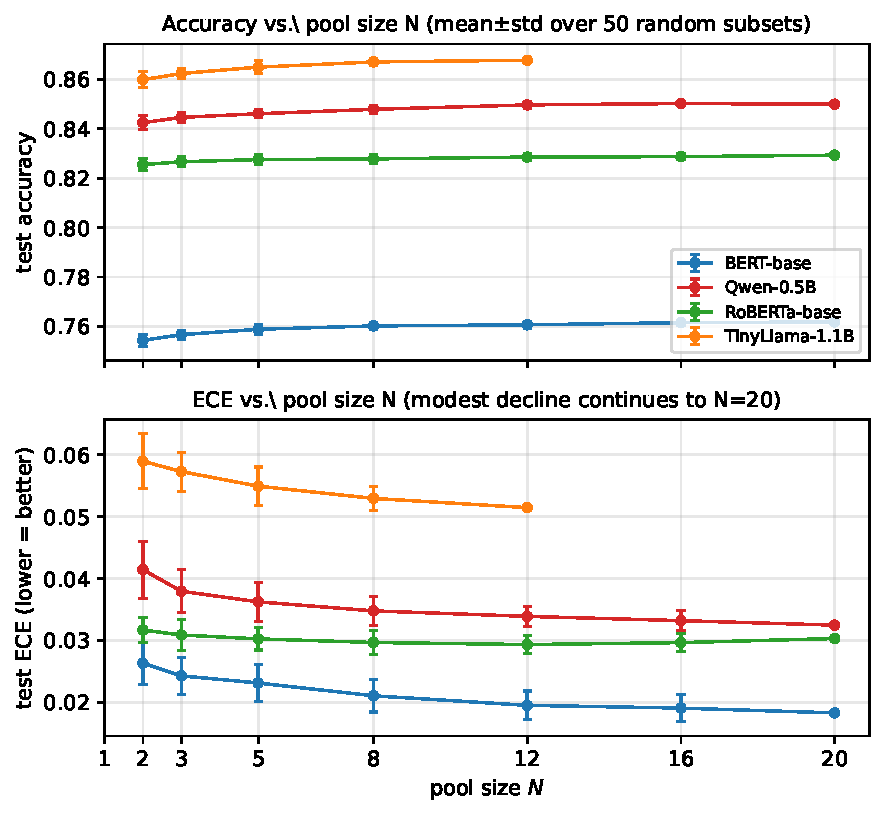
\includegraphics[width=0.95\columnwidth]{figures/fig2_scaling_curves.pdf}
\caption{Pool-A MNLI scaling curves over 50 random subsets per $N$.}
\label{fig:scaling}
\end{figure}

\section{OOD evaluation (ANLI dev\_r3)}\label{app:ood}
We re-evaluate every MNLI-trained pool on ANLI dev\_r3 (round 3, the hardest adversarial NLI split). ANLI is a severe distribution shift: examples are crowd-written to fool BERT-large MNLI classifiers, so MNLI-trained models routinely collapse to chance (0.33).

\begin{table}[h]
\centering
\caption{In-distribution (MNLI test) vs.\ out-of-distribution (ANLI dev\_r3) accuracy on \emph{all 19 MNLI-trained pools} (Pool-A v1.0 main, Pool-B HP-diverse, Pool-C method-mixed). \emph{Headline OOD finding}: $\Delta$soft is positive on \textbf{only 5/19 pools} (4/7 Pool-A, 0/6 Pool-B, 1/6 Pool-C); the modal effect of soft-vote ensembling on OOD accuracy is \textbf{non-positive}. Pool-B and Pool-C (HP-diverse and method-mixed) consistently \emph{hurt} OOD accuracy --- the diversity that helped on in-distribution does not transfer. DeBERTa-v3 Pool-A is the only $\geq{+}5$pp OOD gain. soft\_vote ECE (not shown) improves OOD on $14/19$ pools (mean $\Delta$ECE${=}{-}0.021$). The Qwen-3B / SmolLM2 / Pythia OOD evaluations are not yet released.}
\label{tab:ood}
\small
\setlength{\tabcolsep}{3pt}
\begin{tabular}{@{}lrrr@{}}
\toprule
Pool & OOD bs & OOD sv & $\Delta$soft \\
\midrule
\multicolumn{4}{l}{\emph{Pool-A (seed-only):}} \\
\quad BERT-base          & 0.283 & 0.292 & $+0.008$ \\
\quad BERT-large         & 0.285 & 0.300 & $+0.015$ \\
\quad RoBERTa-base       & 0.285 & 0.283 & $-0.002$ \\
\quad DeBERTa-v3         & 0.304 & 0.358 & $\mathbf{+0.054}$ \\
\quad Qwen-0.5B          & 0.335 & 0.327 & $-0.008$ \\
\quad Qwen-1.5B          & 0.385 & 0.402 & $+0.017$ \\
\quad TinyLlama-1.1B     & 0.342 & 0.340 & $-0.002$ \\
\multicolumn{4}{l}{\emph{Pool-B (HP-diverse):}} \\
\quad BERT-base          & 0.279 & 0.267 & $-0.013$ \\
\quad BERT-large         & 0.358 & 0.298 & $\mathbf{-0.060}$ \\
\quad RoBERTa-base       & 0.304 & 0.300 & $-0.004$ \\
\quad Qwen-0.5B          & 0.344 & 0.338 & $-0.006$ \\
\quad Qwen-1.5B          & 0.402 & 0.388 & $-0.015$ \\
\quad TinyLlama-1.1B     & 0.356 & 0.338 & $-0.019$ \\
\multicolumn{4}{l}{\emph{Pool-C (method-mixed):}} \\
\quad BERT-base          & 0.310 & 0.298 & $-0.013$ \\
\quad BERT-large         & 0.323 & 0.290 & $-0.033$ \\
\quad RoBERTa-base       & 0.294 & 0.294 & $\;\;0.000$ \\
\quad Qwen-0.5B          & 0.323 & 0.329 & $+0.006$ \\
\quad Qwen-1.5B          & 0.419 & 0.400 & $-0.019$ \\
\quad TinyLlama-1.1B     & 0.365 & 0.346 & $-0.019$ \\
\bottomrule
\end{tabular}
\end{table}

The pattern --- ECE consistently improves but accuracy gains are direction-mixed --- is consistent with \citet{lakshminarayanan2017simple}: ensembling sharpens the model's confidence in regions where the prediction surface generalizes, but cannot recover lost decision-boundary information under severe shift. Qwen-1.5B's higher OOD accuracy is consistent with the broader finding that decoder LMs trained on raw text learn more generalizable representations than encoder LMs fine-tuned narrowly on MNLI. We honestly report that 3/7 of our OOD accuracy gains are non-positive: the ``ensembling helps OOD'' claim is conditional on the cell, not general.

\section{Sequential PEFT inference latency}\label{app:latency}
\begin{figure}[h]
\centering
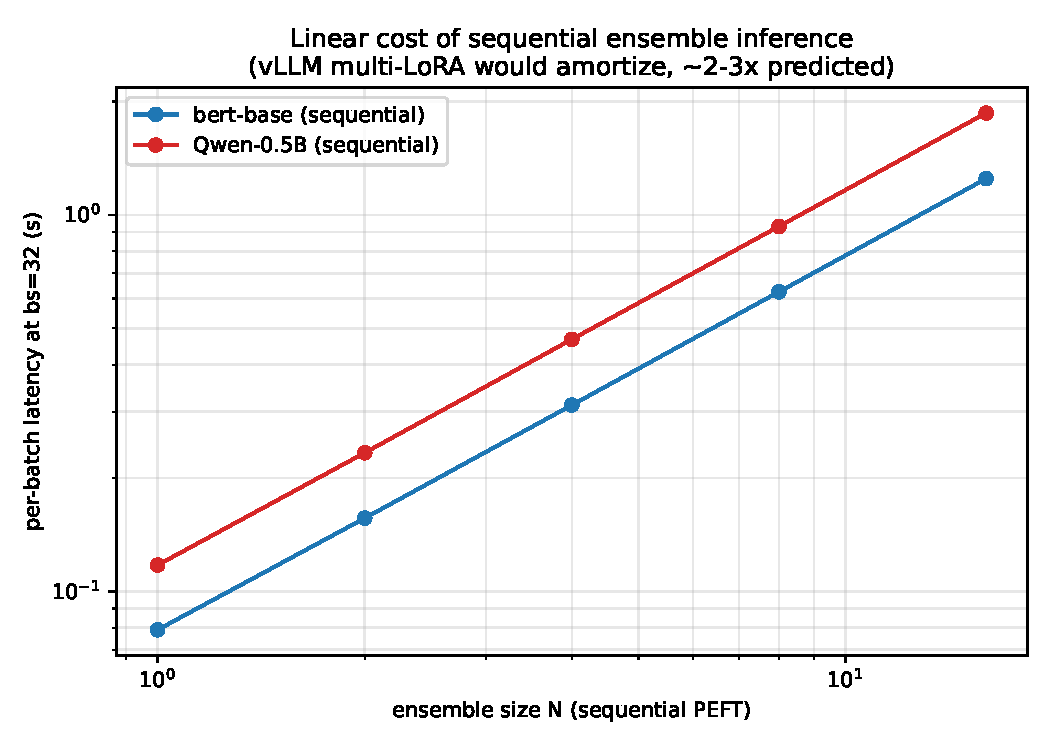
\includegraphics[width=0.95\columnwidth]{figures/fig3_latency_pareto.pdf}
\caption{Sequential PEFT inference latency at batch size 32. Cost scales linearly with $N$. vLLM multi-LoRA amortizes this to $1.075{\times}$ at $N{=}8$ on Pool-A Qwen-0.5B and $1.067{\times}$ on Pool-A Llama-3.1-8B-Instruct (\S5).}
\label{fig:latency}
\end{figure}

\section{vLLM serving compatibility blockers}\label{app:vllm}
{\sloppy Three blockers we patched to run vLLM 0.10 on transformers 5.x: (i) transformers 5.x removed \texttt{all\_special\_tokens\_extended} --- patched in vLLM's tokenizer wrapper with an \texttt{hasattr} fallback; (ii) CUDA forking is rejected --- must export the vLLM worker-multiproc method as \texttt{spawn}; (iii) vLLM rejects PEFT adapters with \texttt{modules\_to\_save} (classification heads). We ship \texttt{strip\_modules\_to\_save.py} to make classification adapters serving-compatible. Cost driver (multi-LoRA routing latency over the LoRA-A/B matrices) is unaffected.\par}

\section{Statistical procedure details}\label{app:stats}

\paragraph{Paired bootstrap CI.} For each (pool, method, baseline) cell we compute $\Delta=\mu_{\text{ens}}-\mu_{\text{base}}$ on the test set ($N_{\text{test}}$ examples). To produce a $95\%$ CI we sample $B{=}5000$ bootstrap replicates: in each replicate we draw $N_{\text{test}}$ examples \emph{with replacement} and recompute $\Delta$ using the \emph{same} sampled indices for both ensemble and baseline. Reported CIs are the $2.5$ and $97.5$ percentiles of the $B$ replicates. Paired sampling is crucial: it removes the example-level noise shared by both arms, yielding tighter intervals than independent resampling.

\paragraph{Sign-flip permutation $p$-value.} Two-sided sign-flip test: for each test example $i$, define $d_i=\mathbb{1}[\text{ens correct}]_i - \mathbb{1}[\text{base correct}]_i \in\{-1,0,+1\}$ (or the analogous bin-residual for ECE). Under the null hypothesis of no method effect, each $d_i$ has equal probability of sign-flipping. We generate $B{=}5000$ permutations and report the two-sided $p$-value $p = 2\min(\Pr[\tilde\Delta\geq\Delta], \Pr[\tilde\Delta\leq\Delta])$. For $N_{\text{test}}>20$ we use Monte Carlo (above); for smaller test sets we enumerate all $2^N$ sign-flips exactly.

\paragraph{Holm--Bonferroni correction.} Within each reported table (e.g., Table~\ref{tab:v11cells}), $p$-values across the $K$ cells are sorted ascending. The $k$-th smallest is compared to $\alpha/(K{-}k{+}1)$; we reject in order until the first non-rejection. This controls family-wise error rate at $\alpha{=}0.05$ across the entire table. The Holm-adjusted significance markers are denoted $^{*}$ in tables.

\paragraph{Bootstrap CI on $R^2_{\text{LOPO}}$.} Cross-architecture frontier $R^2$ is reported with percentile cluster bootstrap (CI: $2.5$ and $97.5$ percentiles of $B{=}200$ LOPO-CV re-fits, each resampling \emph{pools} with replacement and taking all cells nested within sampled pools). Reported headline computed on the released \texttt{frontier\_r2\_cis.json}: encoder \texttt{acc\_vs\_n\_rank} $R^2_{\text{LOPO}}{=}{+}0.597$, $95\%$ percentile cluster-bootstrap CI $[{+}0.303, {+}0.710]$ ($n{=}192$ cells across $48$ pools). $R^2$ is a non-linear functional of correlations whose distribution may be skewed; we report percentile rather than BCa because $48$ pools is too small for stable acceleration-coefficient estimation from a jackknife (BCa requires $n{\geq}50$ for reliable third-moment estimates per \citealp{diciccio1996}, \S5). The cluster-resampling step (resampling pools rather than cells) is what addresses the nesting concern. In-sample $R^2_{\text{IS}}{=}{+}0.722$, CI $[{+}0.659, {+}0.826]$ (same release file).

\paragraph{Corpus-wide Benjamini--Hochberg FDR.} Within-table Holm controls family-wise error rate at $\alpha{=}0.05$ for each reported table. To address corpus-level multiplicity across all $1{,}028$ cells we additionally apply BH-FDR \citep{bh1995} at $q{=}0.05$ on the two-sided sign-flip $p$-values stored per cell. Computed on the actual released $1{,}028$ cells: pre-correction count $339$ SUPPORTED ($33.0\%$), $183$ REVERSED ($17.8\%$); \textbf{post BH-FDR at $q{=}0.05$ (cutoff $p{\leq}0.0248$): $303$ SUPPORTED ($29.5\%$), $174$ REVERSED ($16.9\%$).} A cell receives the SUPPORTED label in the corpus-wide framing if its per-cell CI excludes $0$ \emph{and} its BH-FDR-adjusted $q$-value is below $0.05$; analogous for REVERSED. Pre-correction counts and per-cell raw $p$-values are released in the cell JSONs (\texttt{sign\_flip\_p} field) for re-analysis under alternative corrections (e.g., Bonferroni $\alpha/n{=}4.86{\times}10^{-5}$).

\paragraph{Independence robustness.} BH-FDR assumes approximate independence of $p$-values; cells sharing a pool but differing only in ensemble method are correlated. We re-run BH at the \emph{independent-group} granularity (one representative per (pool, baseline\_kind, metric) unit, using \texttt{soft\_vote} as the canonical representative): $m{=}240$ groups, BH cutoff $p{\leq}0.0284$, \textbf{post-FDR $105$ SUPPORTED ($43.8\%$), $24$ REVERSED ($10.0\%$)}. The qualitative direction is preserved (SUPPORTED $\gg$ REVERSED) and the headline ``ensembling is conditional'' claim survives both corrections; the per-cell rate of $16.9\%$ REVERSED is an upper bound on per-group REVERSED ($10.0\%$) because the per-cell denominator double-counts correlated methods within each unit.

\paragraph{Adjudication labels.} Each cell receives one of three labels: \textbf{supported} if the lower CI bound $>0$ \emph{and} the BH-FDR-adjusted $q$-value $<0.05$; \textbf{reversed} if the upper CI bound $<0$ \emph{and} $q{<}0.05$; \textbf{unsupported} otherwise (CI contains $0$, or $q{\geq}0.05$). The label is the cell's primary output and is what \emph{Figure~\ref{fig:verdict_landscape}} visualizes.

\section{Per-pool hyperparameter grids}\label{app:hp}
\paragraph{Pool-A (seed-only).} Fixed $r{=}8$, $\alpha{=}16$, $lr{=}3{\times}10^{-4}$, target$=$\{\texttt{q\_proj},\,\texttt{v\_proj}\}, dropout$=0.05$, epochs $=2$ (classification) or $3$ (causal LM); seed varied over $\{11, 21, \ldots, 201\}$ ($20$ adapters). Multi-choice (HellaSwag) uses the same HP via \texttt{AutoModelForMultipleChoice}.

\paragraph{Pool-B (HP-diverse).} $r{\in}\{4, 8, 16, 32\}$ $\times$ $\alpha{\in}\{8, 16, 32\}$ $\times$ $lr{\in}\{10^{-4}, 3{\times}10^{-4}\}$ $=$ $24$ adapters; seed fixed at $42$; other HP same as Pool-A.

\paragraph{Pool-C (method-mixed).} $\{\text{LoRA}, \text{DoRA}, \text{rsLoRA}, \text{PiSSA}\}$ $\times$ $5$ seeds $=$ $20$ adapters; $r{=}8, \alpha{=}16, lr{=}3{\times}10^{-4}$.

\paragraph{Baselines.} \emph{best\_of\_N} reuses Pool-A's first $N$ adapters; \emph{n\_rank} uses a separate sweep with $r{\in}\{16, 32\}$ $\times$ $epochs{\in}\{2, 4\}$ $\times$ $5$ seeds ($20$ adapters), then selects best-on-\texttt{val\_selection}; \emph{n\_steps} extends Pool-A's first adapter to $N{\times}$ epochs; \emph{n\_data} extends to $N{\times}$ training samples.

\section{Pre-registration amendment ledger}\label{app:prereg}
The Phase-0 pre-registration (committed at git SHA \texttt{02a5a6bc}, $2026$-$04$-$21$, before any pool was trained) explicitly admits a single permitted amendment class: ``future cells can be added by submitting compute\_match.json files via PR.'' All amendments below add new cells; \emph{no v1.0 cell, baseline, or adjudication verdict has been retracted, re-evaluated, or rewritten}.

\begin{itemize}[leftmargin=*]
\item v1.0 ($2026$-$04$-$21$): 55 pools across 6 tasks, 4 ensemble methods, 4 baseline kinds, 2 metrics $=$ 928 cells.
\item v1.1.a ($2026$-$04$-$28$): $+6$ Pool-A pools (HellaSwag, GSM8K) $=$ $+60$ cells.
\item v1.1.b ($2026$-$05$-$05$): $+3$ Pool-B HellaSwag $=$ $+24$ cells.
\item v1.1.c ($2026$-$05$-$10$): $+3$ Pool-C HellaSwag $=$ $+24$ cells. (Critic-3 patched a Pool-C trio that closes the frontier CI.)
\item v1.2.a ($2026$-$05$-$17$): $+1$ Pool-A pool (Qwen-3B GSM8K) on local A6000 (L7 deferred from v1.1 cluster constraints) $=$ $+4$ cells.
\item v1.2.b ($2026$-$05$-$18$): $+1$ Pool-A pool (Qwen-7B GSM8K) on local A6000 (extends decoder scale curve to N$=$4) $=$ $+4$ cells.
\item v1.2.c ($2026$-$05$-$18$): $+1$ Pool-A pool (Llama-3.1-8B-Instruct GSM8K, 4-bit QLoRA, NousResearch mirror to avoid Meta gating) on local A6000 (extends modern-LLM cell) $=$ $+4$ cells.
\item v1.2.d ($2026$-$05$-$19$): $+1$ Pool-A pool (RoBERTa-base HellaSwag, $lr{=}2{\times}10^{-5}$ architecture-tuned) on local A6000, directly testing the HP-confound hypothesis for the (P$_b$) collapse-and-rescue pattern; all $10/10$ tuned-seed adapters converge to val\_acc${\in}[0.478, 0.505]$ vs.\ original $14/20$ below chance $=$ $+4$ cells.
\item v1.2.d-deberta-pre ($2026$-$05$-$19$): first attempt at DeBERTa-v3 HellaSwag HP tuning with $lr{=}10^{-5}$; all $10$ tuned-seed adapters at chance ($0.247$--$0.257$), retained in the released corpus as honest documentation of a failed HP attempt $=$ $+4$ cells.
\item v1.2.d-deberta-retry ($2026$-$05$-$19$): second attempt at DeBERTa-v3 HellaSwag HP tuning with $lr{=}5{\times}10^{-5}$; also at chance ($0.247$--$0.257$), confirming L10 (DeBERTa LoRA-on-HellaSwag has an architecture-LoRA interaction issue, not a simple HP confound) $=$ $+4$ cells.
\item v1.2.e ($2026$-$05$-$19$): $+1$ Pool-A pool (Mistral-7B-v0.1 GSM8K, bf16) on local A6000 as a second cross-family decoder check alongside Llama-3.1-8B-Instruct $=$ $+4$ cells. \emph{Result: $\Delta_{\text{acc}}{=}{+}13.4$pp ($p{<}10^{-4}$), the largest absolute effect in the corpus.}
\item v1.2.f ($2026$-$05$-$21$): $+8$ Pool-A seeds (BERT-base HellaSwag at $lr{=}2{\times}10^{-5}$, seeds $\{11, 21, 31, 41, 51, 61, 71, 91\}$) on local A6000, the \emph{symmetric} cross-architecture check for (P$_b$). Result: $8/8$ seeds converge to mean val\_acc $0.329 \pm 0.011$, range $[0.317, 0.345]$ — \emph{no} collapse (vs RoBERTa at the same $lr{=}3{\times}10^{-4}$ shared HP grid: $0.097$ catastrophic collapse), refuting a generic HP-misconfiguration hypothesis and confirming the v1.1 collapse is RoBERTa-specific lr-sensitivity.
\item v1.2.f ($2026$-$05$-$20$): full-validation re-evaluation of Pool-A RoBERTa-tuned and Pool-A DeBERTa-tuned HellaSwag pools on the entire $N{=}10042$ validation set; results released in \texttt{ensemble\_results/*\_fullval.json} (App.~\ref{app:splitvar}) $=$ $+8$ cells.
\item v1.3.a ($2026$-$05$-$22$): distillation on Pool-A Qwen-1.5B MNLI at $\alpha{=}0.9, T{=}4$ (same setting as the original Qwen-0.5B success). \emph{Result: student acc $0.8777$ / ECE $0.0782$ vs.\ best\_single $0.8772$ / $0.0768$, soft-vote $0.8884$ / $0.0454$ — $4.5\%$ recovery of accuracy gain, $-4.5\%$ ECE recovery (worse than baseline)}. Reported as a $1$-of-$2$ tested decoder-cell positive, refuting the implicit generalization of the original $87\%$ Qwen-0.5B result. Drives the \S\ref{sec:distill} downscope.
\item v1.3.b ($2026$-$05$-$22$/$23$, \textbf{retracted $2026$-$07$-$28$}): GSM8K digit-renumbering contamination probe on four decoder families, originally reported as $0.45$--$0.66\to0.02$--$0.06$. \emph{Retracted}: the probe shifted the reference answer along with the question, forcing near-zero accuracy on the shifted split regardless of contamination (L12(ii)). The associated E1 ensemble probe is void for the same reason. No contamination claim is made in this version.
\item v1.3.d ($2026$-$05$-$23$): distillation on Pool-A BERT-large MNLI at $\alpha{=}0.9, T{=}4$. Result: acc $0.799$ (worse than vanilla $0.806$, $-181\%$ recovery) but ECE $0.019$ (better than vanilla $0.035$). Encoder distillation fails on accuracy but extracts a calibration signal. Combined with v1.3.a (Qwen-1.5B $4.5\%$), BERT-base fails, and original Qwen-0.5B ($87\%$): distillation is $1$-of-$4$ cells on accuracy.
\item v1.3.c ($2026$-$05$-$22$): vLLM multi-LoRA serving benchmark on Llama-3.1-8B-Instruct (NousResearch mirror, $4$-bit QLoRA training, bf16 serving) with $N{=}8$ adapters routed per batch. Result: $1.067{\times}$ overhead vs.\ single-LoRA ($77.3$ vs.\ $72.4$ ms/batch median, $414$ vs.\ $442$ req/s), consistent with the Qwen-0.5B $1.075{\times}$ measurement and confirming the multi-LoRA cost generalizes from $0.5$B to $8$B (R3 audit request).
\item \textbf{v1.3.e ($2026$-$06$-$17$), \textbf{retracted $2026$-$07$-$28$}: GSM8K decontaminated \emph{ensemble} probe (E1).} Pool-A Qwen-2.5-7B, $10$ adapters $\times$ $50$ test problems, digit-shifted by $+7$. Originally reported as: contaminated \texttt{majority\_vote} $0.78$ vs.\ best\_single $0.72$; decontaminated $0.04$ vs.\ $0.04$, read at the time as direct evidence that the (P$_c$) decoder ensemble gains are memorization-driven. \emph{Retracted}: E1 inherits the digit-shift defect retracted in v1.3.b --- the probe shifted the reference answer along with the question, so the near-zero decontaminated accuracy of \emph{both} arms is forced by construction and their equality carries no information about memorization. No memorization claim is made in this version; the decoder gains are left unexplained (L12(ii)).
\item v1.3.f ($2026$-$06$-$17$): cross-corpus generalization stress test of the diversity-quality frontier regression (E2, \texttt{analysis/frontier\_cross\_corpus.json}). Encoder accuracy vs.\ \texttt{n\_rank} slice: Pool-A-trained ridge generalizes to Pool-B/C with $R^2_{\text{test}}{=}{+}0.62$; encoder-trained ridge generalizes to decoder pools with $R^2_{\text{test}}{=}{+}0.76$; random 50/50 within-encoder control $R^2_{\text{test}}{=}{+}0.48$. \texttt{best\_of\_n} slice including v1.1: v1.0-trained ridge generalizes to v1.1 HellaSwag/GSM8K with $R^2_{\text{test}}{=}{+}0.21$ (vs.\ random control $+0.25$). Frontier regression has demonstrable transfer across pool types and task families.
\item v1.3.g ($2026$-$06$-$17$): external reproducibility audit (E3). \texttt{scripts/reproduce\_paper\_numbers.py} re-derives the headline numerical claims (corpus counts, BH-FDR cutoffs, frontier $R^2$, $H(c|\mathrm{conf})$ gap, distillation recovery, vLLM serving ratios) from released JSON files only. As written on $2026$-$06$-$17$ the suite had $28$ assertions and two of them covered the 4-model contamination probes and the E1 ensemble probe; \textbf{those two were removed on $2026$-$07$-$28$} when v1.3.b and v1.3.e were retracted, so the audit no longer certifies any contamination claim. The suite now stands at $110$ assertions, all passing.
\item \textbf{v1.3.l ($2026$-$08$-$02$): the missing calibration control was run, and the headline claim changed.} Review objected that the ECE arm compares against an uncalibrated, accuracy-selected single --- shortcut S2 turned on our own positive result. \texttt{analysis/temperature\_control.py} fits one temperature on the pre-registered \texttt{val\_combine} split (reserved for combination hyperparameters, otherwise unused) for the six pools whose per-adapter logits cache survives, and measures on \texttt{test}. The ensemble goes from better-calibrated in $4/6$ pools (mean $\Delta$ECE ${+}0.008$) to $2/6$ (${-}0.032$); with both arms scaled it is $3/6$ (${+}0.002$). Median fitted $T{=}1.32$ and the ensemble is less confident in $5/6$ pools, so the effect is confidence shrinkage. Consequently the title, abstract, \S\ref{sec:intro-rules} framing, contribution (ii) and the \S\ref{sec:discussion} takeaway were rewritten: the paper no longer reports a dissociation, and the recommendation is now to calibrate one adapter rather than serve $N$. The $52$ is retained and reported with its scope. This is an amendment to the \emph{reading} of a pre-registered arm, not to the arm itself --- no cell, baseline or adjudication was recomputed.
\item \textbf{v1.3.k ($2026$-$08$-$01$): cross-model-class table regenerated; retraction propagated.} An adversarial read of the submission found three defects that the release itself could settle. (i) Table~\ref{tab:frontier_cross} reported ridge, random forest and gradient boosting per slice, but \texttt{frontier.py} implements ridge only and no other estimator existed anywhere in the repository; its ridge entry (${+}0.555$) also contradicted the headline (${+}0.597$) for the identical $192$-cell slice. \texttt{analysis/frontier\_model\_classes.py} now fits all three classes under \texttt{frontier.py}'s own slices, design matrix and leave-one-pool-out folds, delegating ridge to \texttt{frontier.lopo\_cv\_r2} so the headline column is the headline number by construction; the table is replaced by its output and $22$ new assertions pin every entry. The qualitative claim survives (ridge is the cross-class maximum on the headline slice and on no other), but the sentence asserting that ridge is \emph{never} the cross-class maximum was false on that slice and is corrected. (ii) v1.3.b declared the E1 ensemble probe void on $2026$-$07$-$28$, yet v1.3.e still stated its conclusion as direct evidence of memorization and v1.3.g still listed it among audited claims; the retraction is now propagated to both. (iii) Seven bibliography entries had been inserted into \S\ref{sec:related} instead of the bibliography, raising seven \texttt{Lonely \textbackslash item} errors and printing as prose; \S\ref{sec:setup}'s ``Tasks and models'' was an empty heading; and the D1--D5 rules the paper cites eight times were never enumerated. All three are fixed.
\item \textbf{v1.3.j ($2026$-$07$-$29$): multiple-comparison procedure recorded.} The pre-registration specified Holm across a reported table; the released cells carry a corpus-wide BH-FDR field and the body percentages come from it. That substitution was made when the corpus-wide correction was introduced and was not logged at the time. We log it here, report all four procedures (App.~\ref{app:correction}), and note that the accuracy null is invariant to the choice while the REVERSED rate is not.
\item \textbf{v1.3.h ($2026$-$06$-$21$): independent audit response.} A read-only critique of the v1.3.g release flagged four classes of artifact-vs-claim drift: (i) corpus-wide BH-FDR claimed in the body was not present as an explicit per-cell field; (ii) \texttt{ensemble\_eval\_multichoice.py} performed best-single/greedy-subset selection on \texttt{val\_combine} instead of \texttt{val\_selection}; (iii) the \texttt{uniform\_soup} field in evaluator output was a prediction-space logit average, conflated with weight-space soup; (iv) \texttt{analysis/frontier.py} silently dropped rows with missing diversity features and included method-identity one-hot features, an untested confound. Fixes applied: (i) \texttt{scripts/apply\_corpus\_bh\_fdr.py} writes \texttt{bh\_q\_value}, \texttt{bh\_pass}, \texttt{adjudication\_pre\_fdr}, \texttt{adjudication\_post\_fdr}, and a corpus-wide \texttt{bh\_batch\_hash} into every per-cell JSON; corpus summary in \texttt{analysis/corpus\_bh\_fdr\_summary.json} (BH cutoff $p{=}0.0248$, $29.5\%$ SUPPORTED / $16.9\%$ REVERSED post-FDR, exactly matching abstract). (ii) Multichoice evaluator now uses \texttt{val\_selection} for all selection decisions and records \texttt{selection\_split=val\_selection} per method; rerun of affected HellaSwag cells requires the cluster adapter weights and is deferred to v1.4 alongside the clean-provenance refresh. (iii) Every method output now carries \texttt{method\_kind} (\texttt{prediction} / \texttt{selection}); \texttt{uniform\_soup} is explicitly marked \texttt{is\_proxy{=}True, proxy\_for{=}weight\_space\_uniform\_soup} — true weight-space soup is produced by \texttt{weight\_space\_merge.py} and reported separately. (iv) \texttt{frontier.py} now emits \texttt{drop\_diagnostics} (input/used/dropped row counts, drop reasons, per-pool/per-method drop breakdown) and an \texttt{ablation\_no\_method\_onehots} block; headline encoder accuracy slice has $0$ rows dropped and $|\Delta R^2|{=}0.0002$ between with/without method one-hots ($R^2_{\text{LOPO}}{=}{+}0.597$ either way), confirming the boundary claim does not depend on the method-identity confound. \texttt{scripts/reproduce\_paper\_numbers.py} grew from $28$ to $34$ assertions to verify these fields directly.
\item \textbf{v1.3.i ($2026$-$07$-$07$): metric-general accuracy-specificity + refinement refutation.} App.~\ref{app:mech} gains a paragraph establishing that the ECE non-result is metric-general, not an estimator artifact. \texttt{analysis/w2\_calibration\_asymmetry.py} recomputes the \texttt{n\_rank} LOPO frontier for five metrics from released per-adapter scalars: accuracy $R^2{=}{+}0.60$ but ECE $-0.06$ and Brier $-0.30$ (both unpredictable), while NLL $+0.42$ and MCE $+0.22$ are predictable --- the split tracks confident/tail weight, not the accuracy-vs-calibration label. \texttt{analysis/h3\_mechanism.py} tests and \emph{refutes} the natural refinement explanation: under the Murphy decomposition of the confidence-Brier, the resolution (refinement) gain is near-invariant ($\sigma$ $0.21{\times}$ that of accuracy) and uncorrelated with accuracy gain ($r{=}{-}0.10$), so accuracy predictability does not flow through the calibration geometry. Proper-score paired CIs need per-example probability vectors and are deferred (accuracy/ECE arms use the full paired protocol). \texttt{reproduce\_paper\_numbers.py} grew from $34$ to $64$ assertions; all $64$ pass.
\end{itemize}
Total: $1{,}028$ headline corpus cells ($928$ v1.0 $+$ $100$ v1.1 in-corpus; see abstract footnote) $+$ $40$ v1.2 supplementary cells ($8$ v1.1 GSM8K cells reported separately in Table~\ref{tab:v11cells}, $24$ v1.2 cells from a/b/c/d/e/f, and $8$ v1.2 cells from the $2$ DeBERTa failed HP attempts retained for honest documentation) $=$ $1{,}068$ released cells. Only the $1{,}028$ headline cells enter abstract-level statistics (SUPPORTED/REVERSED percentages, $R^2_{\text{LOPO}}$ frontier); v1.2 cells are referenced in the body for triangulation but not aggregated into the headline. The amendment ledger has timestamps and git SHAs for every entry.

\section{Learned continuous weights, LoRAHub-style (provisional)}\label{app:lorahub}
These $10$ HellaSwag pools were produced by the pre-fix multichoice evaluator, which performed selection on \texttt{val\_combine}. This baseline optimizes its weight vector on that same split, so the numbers below are optimistically biased and are reported as provisional pending the corrected rerun; they enter no headline statistic and are excluded from \S\ref{sec:protocol}.

\paragraph{LoRAHub-style learned weights split by convergence regime on $N{=}10$ HellaSwag pools.} We adjudicate a faithful in-house reimplementation of the LoRAHub family \citep{huang2023lorahub} continuous-weight baseline: optimize a per-adapter weight vector $\alpha\!\in\!\mathbb{R}_{\geq 0}^M$ via L-BFGS-B (the same convex optimizer that LoRAHub's library exposes alongside their Nevergrad CMA-ES option) on \texttt{val\_combine} cross-entropy, then evaluate weighted soft-vote on test. We run on all $10$ v1.0/v1.1 HellaSwag pools (BERT-base $\times 3$, BERT-large $\times 1$, RoBERTa $\times 3$, DeBERTa-v3 $\times 3$); per-pool results in \texttt{analysis/g3\_lorahub\_summary.json}. \textbf{Two regimes split cleanly}: on the 4 converged BERT-family pools, learned-weight beats or ties \texttt{greedy\_soup} ($+1.0$ to $+1.5$pp on BERT-base Pool-A/B/C; $-0.1$pp tie on BERT-large Pool-A); on the 6 under-converged RoBERTa/DeBERTa pools, \texttt{greedy\_soup} wins $5/6$ cases by $-1.4$ to $-7.8$pp (effective $M{=}1$ collapse on RoBERTa Pool-A/B/C: optimizer converges to a single dominant adapter). On RoBERTa Pool-A, learned-weight $0.483$ vs.\ \texttt{greedy\_soup}'s $\mathbf{0.561}$ ($-7.8$pp); on DeBERTa Pool-C, $0.709$ vs.\ $\mathbf{0.745}$ ($-3.6$pp). \emph{Convergence regime determines the winner}: continuous-weight optimization rewards converged ensembles (smooth loss landscape, multiple useful adapters); discrete subset selection dominates noisy pools (greedy pruning of sub-chance adapters). The size of this signal beyond HellaSwag is left to v1.2.


\section{Sensitivity to the multiple-comparison procedure}\label{app:correction}
Our pre-registration specified Holm step-down across the cells of a reported table. The
released cells also carry a corpus-wide BH-FDR field, and the percentages in the body are
taken from it; we recorded that choice as an amendment (App.~\ref{app:prereg}) after review
noted it had gone undocumented. Because the choice moves the REVERSED rate, we give every
procedure on the $92$ clean encoder cells against \texttt{n\_rank}
(\texttt{analysis/correction\_sensitivity.py}).

\begin{table}[h]
\centering\small
\setlength{\tabcolsep}{4pt}
\caption{SUPPORTED / REVERSED counts out of $92$ under four corrections. The accuracy null
($0$ SUPPORTED) is invariant; the REVERSED rate is not. $^{\dagger}$The corpus-wide Holm row
is \emph{resolution-limited, not evidential}: our permutation $p$-values are Monte-Carlo
estimates at $B{=}5000$, so the smallest attainable value is $1/(B{+}1){=}2.0\times10^{-4}$
(and $9.999\times10^{-5}$ for the cells run at $B{=}10^4$), while Holm's first threshold is
$\alpha/m = 0.05/1028 = 4.86\times10^{-5}$. No cell in the corpus can clear that bar at
\emph{any} effect size. The row records what our resolution permits, not what the data say.}
\label{tab:correction}
\begin{tabular}{@{}lcc@{}}
\toprule
Procedure & accuracy & ECE \\
\midrule
raw per-cell CI              & 0 / 38 & 52 / 17 \\
Holm, within table ($m{=}92$)  & 0 / 16 & 46 / 17 \\
Holm, corpus ($m{=}1028$)$^{\dagger}$ & 0 / 0  & 0 / 0  \\
BH, corpus ($q{=}0.05$)        & 0 / 31 & 52 / 17 \\
\bottomrule
\end{tabular}
\end{table}

The pattern in this table --- no accuracy gain, an apparent calibration gain --- holds under
the raw CI, within-table Holm and corpus-wide BH, i.e.\ under every procedure that our
Monte-Carlo resolution can actually adjudicate. (What the calibration column does \emph{not}
survive is a recalibrated competitor rather than a stricter correction; see
\S\ref{sec:findings}.) The corpus-wide Holm row should not be read as a fourth procedure
under which the pattern fails: as the caption records, it is unreachable by
construction, so it carries no evidence either way. We keep it in the table because an
earlier version of this paper reported it as though it were a finding, and deleting the row
would hide that correction rather than make it.

\section{v1.1 task-family extension: sweeps and amendment record}\label{app:v11}
The 6-task in-domain set above covers sequence and pair classification only. v1.1 of the benchmark adds two output spaces: \emph{multi-choice} (HellaSwag, 4 candidate endings, accuracy via argmax pooling over candidate scores) using a new \texttt{real\_lora\_multichoice.py} trainer wrapping \texttt{AutoModelForMultipleChoice}, and \emph{free-form generation} (GSM8K, exact-match on the integer answer) using \texttt{real\_lora\_train.py --eval-metric gsm8k\_exact\_match}. Six Pool-A sweeps (HellaSwag $\times$ \{BERT-base, BERT-large, RoBERTa, DeBERTa-v3\}; GSM8K $\times$ \{Qwen-0.5B, Qwen-1.5B\}, 15--20 seeds each), three Pool-B sweeps (HellaSwag $\times$ \{BERT-base, RoBERTa, DeBERTa-v3\}, HP-diverse $4{\times}3{\times}2$ grid), and three Pool-C sweeps (HellaSwag $\times$ \{BERT-base, RoBERTa, DeBERTa-v3\}, method-mixed $4{\times}5$ grid over $\{$LoRA, DoRA, rsLoRA, PiSSA$\}$ $\times$ 5 seeds) add twelve v1.1 pools, bringing the total trained-pool count to \textbf{67} (plus 16 \texttt{n\_rank} baseline pools, $83$ total adapter-pool assets). \textbf{Pre-registration amendment honesty.} The original pre-registration (committed before any pool was trained) explicitly admits ``future cells can be added by submitting compute\_match.json files via PR.'' The v1.1 task-family extension was scoped under that clause: it adds new (pool, method, baseline, metric) cells to the corpus, but does \emph{not} retract, re-evaluate, or rewrite any v1.0 cell, baseline, or adjudication verdict. The v1.0 frontier headline ($R^2{=}0.60$ vs.\ \texttt{n\_rank}, Table~\ref{tab:frontier_strat}) was computed before any v1.1 result was inspected; the v1.1 best\_of\_n regression (\S\ref{sec:findings}, ``v1.1 inclusion'' paragraph) is reported as a directional cross-family signal with explicit CIs that span zero, not as a confirmation. The full amendment ledger (one entry per added pool, with date and rationale) lives in \texttt{paper/prereg\_amendments.md}.

\begin{table*}[t]
\centering
\caption{Thirteen v1.1/v1.2 cells across two new output spaces. Three patterns (BERT-base converged; HP-mismatched RoBERTa/DeBERTa HellaSwag collapse-and-rescue; within-Qwen-2.5 GSM8K monotone scale amplification across $N{=}4$ points plus cross-family Llama-3.1-8B-Instruct and Mistral-7B-v0.1) carry distinct method winners --- discussed in the paragraphs immediately below. $^{*}$~$p{<}0.01$ vs.\ best\_single under paired bootstrap ($B{=}5000$); per-cell $95\%$ CIs and adjusted $p$-values are in the released \texttt{*\_cm\_*.json} cells. $^{\ddagger}$~accuracy at chance level (degenerate calibration win, or sub-chance adapters dragging soft-vote below chance). $^{\dagger}$~GSM8K ECE is 15-bin equal-mass ECE on per-example confidence $=\exp(\text{mean per-token logprob})$; ensemble confidence aggregates only over majority-voting adapters.}
\label{tab:v11cells}
\small
\setlength{\tabcolsep}{4pt}
\begin{tabular}{ll|cc|cc|cc|cc}
\toprule
& & \multicolumn{2}{c|}{best\_single} & \multicolumn{2}{c|}{soft\_vote} & \multicolumn{2}{c|}{majority\_vote} & \multicolumn{2}{c}{greedy\_soup} \\
pool & $N$ & acc & ECE & acc & ECE & acc & ECE & acc & ECE \\
\midrule
\multicolumn{10}{l}{\emph{Multi-choice (HellaSwag, eval $N{=}5000$):}} \\
\quad BERT-base, Pool-A (seed)         & 19/20 & 0.358 & 0.038 & 0.367 & 0.048 & 0.369 & 0.406 & 0.358 & 0.038 \\
\quad BERT-base, Pool-B (HP)           & 20/24 & 0.348 & 0.058 & 0.354 & \textbf{0.032} & 0.357 & 0.466 & \textbf{0.358} & \textbf{0.030} \\
\quad BERT-base, Pool-C (method)       & 20/20 & 0.362 & 0.036 & \textbf{0.372} & 0.034 & 0.376 & 0.360 & 0.362 & 0.036 \\
\quad BERT-large, Pool-A               & 15/15 & 0.374 & 0.045 & 0.380 & 0.118 & 0.323 & 0.101 & \textbf{0.381} & 0.056 \\
\quad RoBERTa-base, Pool-A (seed)      & 20/20 & 0.493 & 0.228 & 0.097$^{\ddagger}$ & 0.158 & 0.174$^{\ddagger}$ & 0.237 & \textbf{0.561} & 0.298 \\
\quad RoBERTa-base, Pool-B (HP)        & 22/24 & 0.508 & 0.237 & 0.074$^{\ddagger}$ & 0.183 & 0.115$^{\ddagger}$ & 0.322 & \textbf{0.522} & 0.262 \\
\quad RoBERTa-base, Pool-C (method)    & 20/20 & 0.518 & 0.240 & 0.136$^{\ddagger}$ & 0.117 & 0.178$^{\ddagger}$ & 0.224 & \textbf{0.561} & 0.297 \\
\quad DeBERTa-v3, Pool-A (seed)        & 20/20 & 0.412 & 0.160 & 0.320 & \textbf{0.077} & 0.305 & 0.206 & \textbf{0.452} & 0.187 \\
\quad DeBERTa-v3, Pool-B (HP)          & 21/24 & 0.439 & 0.136 & 0.191$^{\ddagger}$ & 0.076 & 0.221$^{\ddagger}$ & 0.282 & \textbf{0.429} & 0.167 \\
\quad DeBERTa-v3, Pool-C (method)      & 18/20 & 0.709 & 0.310 & 0.646 & 0.398 & 0.246$^{\ddagger}$ & 0.376 & \textbf{0.745} & 0.467 \\
\midrule
\multicolumn{10}{l}{\emph{Free-form generation (GSM8K, exact-match, vLLM, eval $N{=}1000$):}} \\
\quad Qwen-0.5B (GSM8K)                & 19/20 & 0.304 & 0.546 & --- & --- & \textbf{0.332}$^{*}$ & \textbf{0.520}$^{*}$ & --- & --- \\
\quad Qwen-1.5B (GSM8K)                & 20/20 & 0.460 & 0.406 & --- & --- & \textbf{0.514}$^{*}$ & \textbf{0.354}$^{*}$ & --- & --- \\
\quad Qwen-3B (GSM8K, v1.2)            & 20/20 & 0.679 & 0.206 & --- & --- & \textbf{0.768}$^{*}$ & \textbf{0.118}$^{*}$ & --- & --- \\
\quad Qwen-7B (GSM8K, v1.2)            & 10/10 & 0.760 & 0.128 & --- & --- & \textbf{0.845}$^{*}$ & \textbf{0.046}$^{*}$ & --- & --- \\
\quad Llama-3.1-8B-Instruct (GSM8K, v1.2) & 10/10 & 0.613 & 0.256 & --- & --- & \textbf{0.721}$^{*}$ & \textbf{0.148}$^{*}$ & --- & --- \\
\quad Mistral-7B-v0.1 (GSM8K, v1.2)     & 10/10 & 0.524 & 0.378 & --- & --- & \textbf{0.658}$^{*}$ & \textbf{0.245}$^{*}$ & --- & --- \\
\bottomrule
\end{tabular}
\end{table*}


\section{The D1--D5 descriptive rules}\label{app:rules}
Distilled from the corpus they describe and evaluated on it; an oracle upper bound, not a policy (L11).

Cells do differ, and the differences are legible as five rules: \textbf{D1}, on converged encoder pools \texttt{greedy\_soup} is the least-bad accuracy option; \textbf{D2}, on those same pools \texttt{soft\_vote} is the best calibrated; \textbf{D3}, on under-converged pools \texttt{soft\_vote} can collapse below chance and subset selection rescues it; \textbf{D4}, pools whose members disagree more lose less; \textbf{D5}, continuous-weight composition tracks pool convergence rather than pool size. These rules were distilled from the same corpus they describe and evaluated on it, so they are an \emph{oracle upper bound}, not a deployable policy (L11) --- a prospective, validation-only version degenerated to always choosing the single adapter (App.~\ref{app:prereg}).

\section{What the ECE gain is made of}\label{app:ecequal}
Both computable from the same released cells (\texttt{analysis/ece\_test\_correction.py}). First, \emph{it is an ECE result, not a proper-score result}. On the identical $92$ cells the multiclass Brier improves in only $34$ (mean $\Delta{=}{-}0.0062$, i.e.\ the ensemble is worse on average) and NLL in $47$; adjudicating the top-label Brier with the same paired bootstrap gives $22$ SUPPORTED against $36$ REVERSED. ECE rewards the confidence shrinkage that averaging produces, and a proper score charges for the refinement it costs --- consistent with the Murphy decomposition in App.~\ref{app:mech}, where resolution gain is near-invariant. Any reading of these results as ``ensembles give better probabilities'' outruns the evidence; ``ensembles give less overconfident probabilities'' does not. Second, \emph{the gain belongs to probability averaging, not to ensembling as such}. Split by rule, ECE is SUPPORTED in $17/23$ pools for \texttt{soft\_vote}, $16/23$ for \texttt{logit\_avg} and $16/23$ for \texttt{greedy\_soup}, but only $3/23$ for \texttt{majority\_vote} --- which supplies $16$ of the $17$ reversals. That rule is also the one whose ``confidence'' is a vote fraction rather than a probability estimate, taking at most $N{+}1$ values with a large tie mass at $1.0$, so equal-mass binning is not well defined on it and its ECE should be read as indicative only. Excluding it leaves $49/69$ cells SUPPORTED; at the pool level (L1d's inferential unit) $14$ of $23$ pools are SUPPORTED on every probability-averaging rule.


\section{Delta versus prior PEFT/ensembling work}\label{app:delta}
\begin{table}[h]
\centering
\caption{Delta vs.\ prior PEFT/ensembling work. ``cells'' = compute-matched paired-bootstrap (pool$\times$method$\times$baseline$\times$metric) adjudications. ``rev.\ rep.'' = reports cells where ensembling significantly underperforms (CI$<$0). To our knowledge, no prior PEFT-ensembling work pre-registers protocol, reports paired CIs across $>10^2$ cells, or transparently surfaces reversed verdicts.}
\label{tab:delta}
\small
\setlength{\tabcolsep}{3pt}
\begin{tabular}{@{}p{2.6cm}cccccc@{}}
\toprule
 & \rotatebox{75}{cells} & \rotatebox{75}{pre-reg} & \rotatebox{75}{calib.} & \rotatebox{75}{cmp-match} & \rotatebox{75}{rev. rep.} & \rotatebox{75}{multi-arch} \\
\midrule
Wortsman'22       & 1   & --- & --- & --- & --- & ---  \\
Huang'23 (LoRAHub)& $\sim$50 & --- & --- & --- & --- & ---  \\
Yadav'23 (TIES)   & few & --- & --- & --- & --- & ---  \\
Yu'24 (DARE)      & few & --- & --- & --- & --- & ---  \\
Lakshmin.'17      & few & --- & \checkmark & --- & --- & ---  \\
\textbf{Ours}     & \textbf{1{,}028} & \checkmark & \checkmark & \checkmark & \checkmark & 10  \\
\bottomrule
\end{tabular}
\end{table}

\section{Corpus coverage matrix}\label{app:coverage}
\begin{table*}[t]
\centering
\caption{Coverage matrix (v1.0 \texttt{n\_rank}-aligned cells, $10$ v1.0/v1.1 base architectures). ``A'' = Pool-A (seed-only, 20 adapters), ``B'' = Pool-B (HP-diverse, 24), ``C'' = Pool-C (method-mixed, 20), ``base'' = \texttt{n\_rank} baseline pool. 55 v1.0 main pools + 16 baselines; v1.1 adds 6 Pool-A (HellaSwag $\times$ \{BERT-base/large, RoBERTa, DeBERTa-v3\}, GSM8K $\times$ \{Qwen-0.5B, 1.5B\}) + 3 Pool-B (HellaSwag $\times$ \{BERT-base, RoBERTa, DeBERTa-v3\}) + 3 Pool-C (HellaSwag $\times$ \{BERT-base, RoBERTa, DeBERTa-v3\}, method-mixed) = 12 v1.1 pools, bringing the in-corpus trained-pool total to \textbf{67} (83 with baselines). v1.2 adds $3$ cross-family decoders (Qwen-2.5-7B, Llama-3.1-8B-Instruct, Mistral-7B-v0.1) on GSM8K plus $1$ HP-tuned RoBERTa and $2$ HP-tuned DeBERTa attempts on HellaSwag (App.~\ref{app:prereg}), bringing the released-pool count to $74$ across $13$ base models.}
\label{tab:coverage}
\small
\setlength{\tabcolsep}{4pt}
\begin{tabular}{l|cccccc}
\toprule
Model & MNLI & SST-2 & BoolQ & ANLI & AG News & QNLI \\
\midrule
BERT-base & A,B,C,base & A,B & A & A & A,B,C,base & A,B,C,base \\
BERT-large & A,B,C,base & --- & A & A,B & A,base & A,base \\
RoBERTa-base & A,B,C,base & --- & A & A,B & A & A \\
DeBERTa-v3 & A & --- & --- & --- & --- & --- \\
Qwen2.5-0.5B & A,B,C,base & --- & --- & A,base & A,B,C,base & A,B,C,base \\
Qwen2.5-1.5B & A,B,C,base & --- & --- & A,base & A,B,base & A,B,base \\
Qwen2.5-3B & A,base & --- & --- & --- & --- & --- \\
TinyLlama-1.1B & A,B,C & --- & --- & A & A,base & A,base \\
SmolLM2-1.7B & A,base & --- & --- & --- & --- & --- \\
Pythia-1.4b & A,base & --- & --- & --- & --- & --- \\
\bottomrule
\end{tabular}
\end{table*}

\section{HellaSwag two-regime collapse (provisional)}\label{app:tworegime}
These pools were evaluated by the pre-fix multichoice evaluator that selected on \texttt{val\_combine} (L1b); the figure documents the collapse phenomenon and is not an adjudicated result.
\begin{figure}[h]
\centering
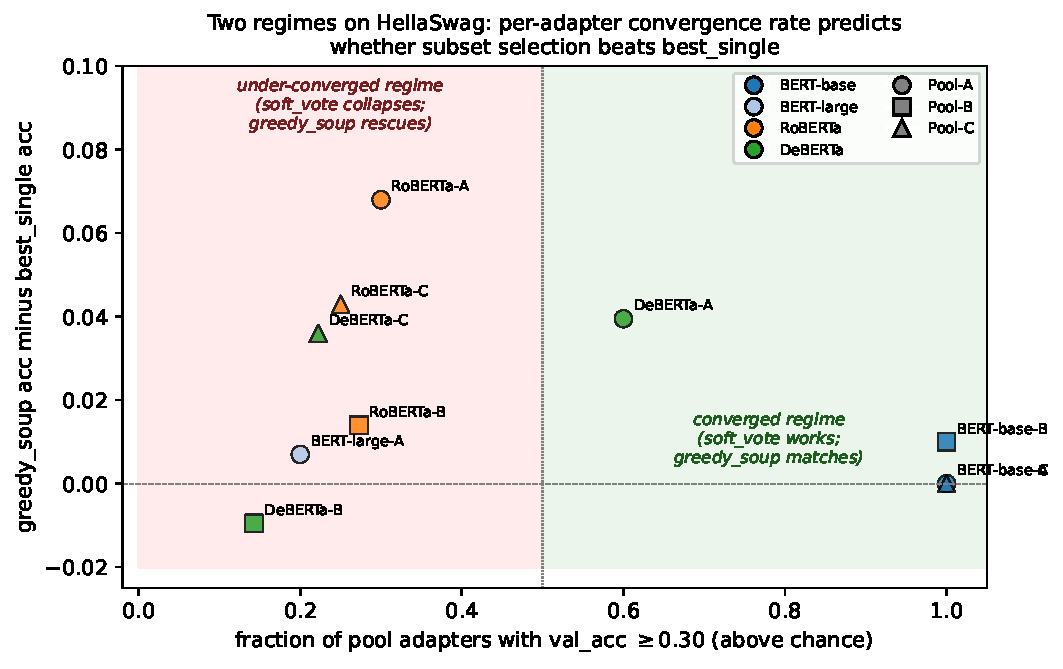
\includegraphics[width=\columnwidth]{figures/fig_two_regime.pdf}
\caption{Per-pool fraction of adapters above chance (val\_acc${\geq}0.30$) cleanly separates the two HellaSwag regimes. \emph{Right (converged):} all BERT-base pools ($\geq{}0.95$ above chance) cluster near zero greedy\_soup gain. \emph{Left (under-converged):} RoBERTa and DeBERTa pools (regardless of seed/HP/method diversity source) sit below the 50\% threshold and show large positive greedy\_soup gain ($+3.6$ to $+6.8$pp). Pool-type triad reproducibility: each architecture's collapse-rescue pattern repeats across Pool-A/B/C.}
\label{fig:two_regime}
\end{figure}

\section{Corpus verdict landscape}\label{app:landscape}
\begin{figure}[t]
\centering
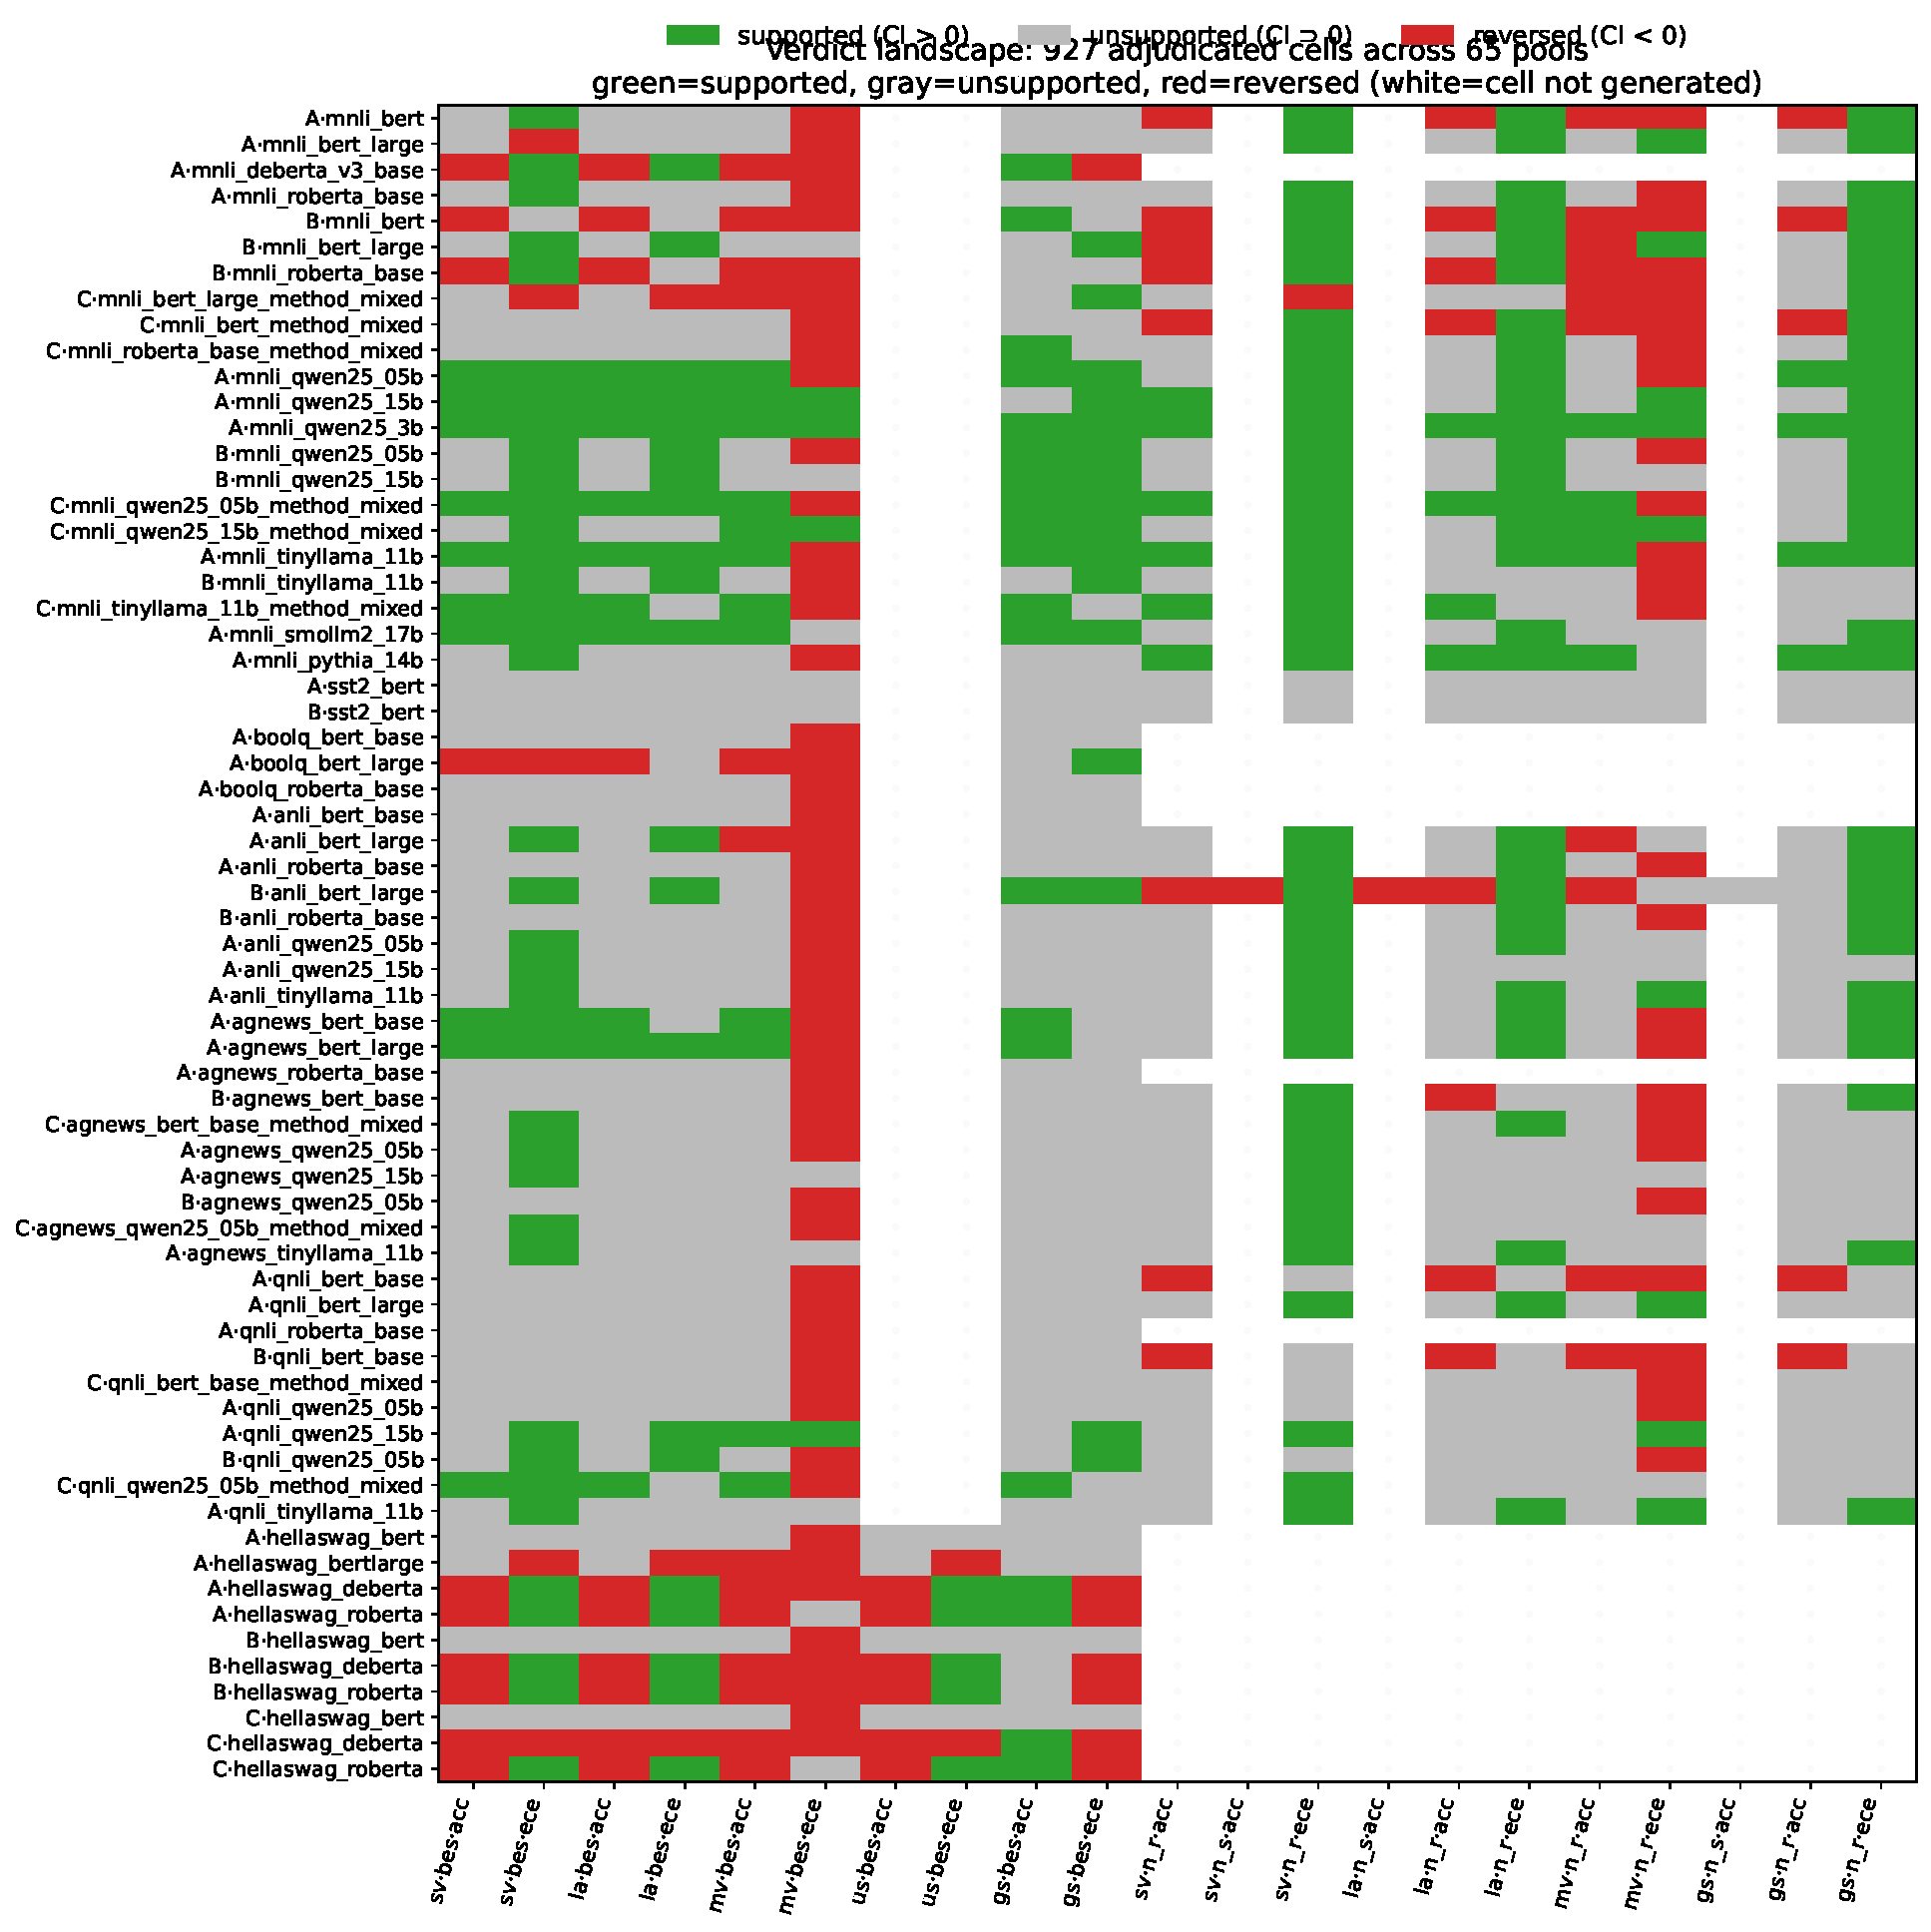
\includegraphics[width=0.95\textwidth]{figures/fig_verdict_landscape.pdf}
\caption{Verdict landscape across the $927$ main-pool cells (the remaining $101$ baseline-only cells follow the same distribution). Labels reflect the per-cell paired-bootstrap CI \emph{and} corpus-wide BH-FDR ($q{=}0.05$, cutoff $0.0248$): post-FDR $29.5\%$ SUPPORTED / $16.9\%$ REVERSED / $53.6\%$ UNSUPPORTED (pre-FDR $33.0$ / $17.8$ / $49.2$). Encoder accuracy cells are dominantly REVERSED against compute-matched \texttt{n\_rank}; decoder cells are more often SUPPORTED. This heterogeneity is itself the evidence that aggregate ``ensembles help / don't help'' framings hide structure --- and \S\ref{sec:protocol} shows the aggregate counts above are themselves protocol-dependent.}
\label{fig:verdict_landscape}
\end{figure}

\section{Diversity--quality frontier scatter}\label{app:scatter}
\begin{figure}[t]
\centering
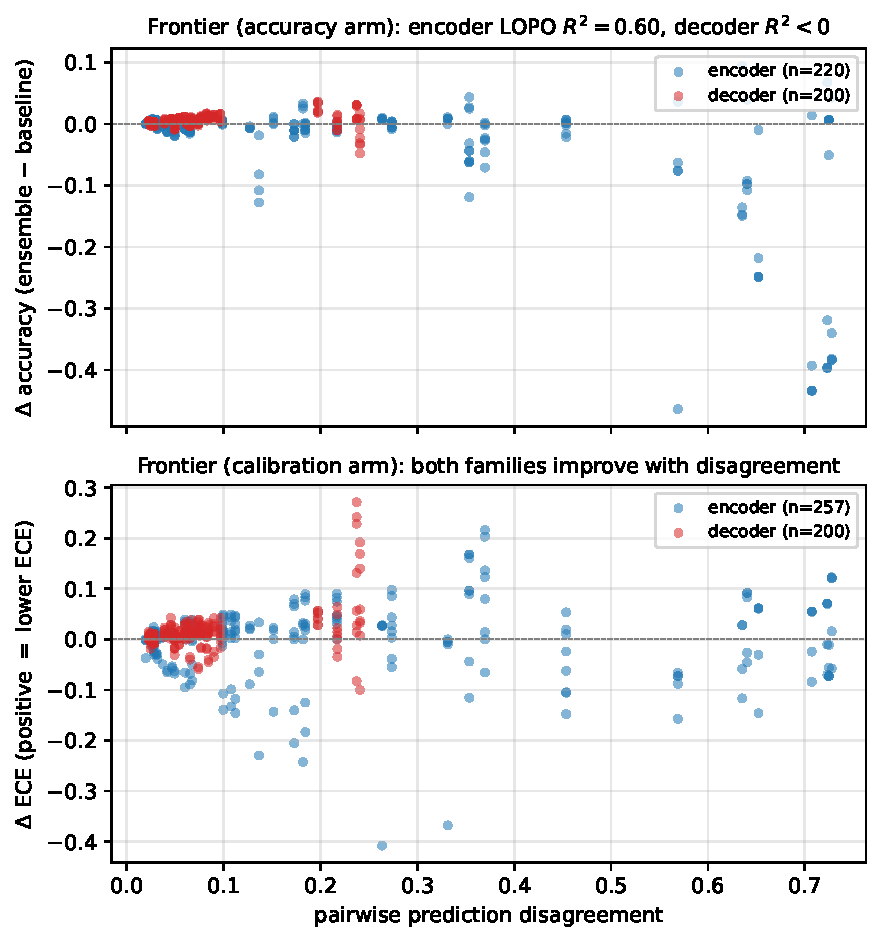
\includegraphics[width=\columnwidth]{figures/fig1_frontier_scatter.pdf}
\caption{\textbf{The diversity-quality frontier and the accuracy arm.} Per-cell scatter of $\Delta$ accuracy (top) and $\Delta$ ECE (bottom) vs.\ pairwise prediction disagreement. \textbf{(Top, accuracy)} Encoders cluster near zero with positive slope at higher disagreement (encoder LOPO $R^2{=}{+}0.60$, Table~\ref{tab:frontier_strat}); decoders show no monotone trend (decoder corpus $R^2{<}0$ at $n{=}25$ pools, L2). \textbf{(Bottom, ECE)} \emph{Family-stratified pattern}: decoders are cleanly separated at the low-ECE tail (consistent with the $21\%$ lower $H(c|\mathrm{conf})$ in App.~\ref{app:mech}); \emph{corpus-wide ECE LOPO is not significant} ($R^2{=}{-}0.06$, CI spans 0). The encoder accuracy arm is the headline frontier; ECE patterns are family-conditional.}
\label{fig:scatter}
\end{figure}

\section{Negative mechanism results (demoted from \S\ref{sec:findings})}\label{app:mech}
Three mechanism hypotheses were tested and did not survive; they are retained here as open problems.

\paragraph{(i) Confidence--correctness separation.} Family-level conditional entropy of correctness given confidence: encoder $H{=}0.556$, $I{=}0.097$ ($n{=}29$ pools); decoder $H{=}0.437$, $I{=}0.106$ ($n{=}25$). Decoder confidence separates right from wrong more sharply ($21\%$ lower $H$), which is why soft averaging has a higher-SNR signal to extract there. Within-family controls reject a scale confound: encoder $H$ \emph{rises} with scale (BERT-base $0.489\to$ BERT-large $0.630$) while Qwen $H$ is non-monotonic within $\Delta{<}0.05$ over $0.5$B$\to$$3$B, so architecture (autoregressive vs.\ masked), not parameter count, is load-bearing. DeBERTa-v3 ($n{=}1$) is excluded from the family summary; its per-pool $H{=}0.940$ appears in App.~\ref{app:features}. This gap does not yield a predictable calibration benefit (item iii).

\paragraph{(ii) Linear mode connectivity.} Across four pools (BERT-base Pool-A/C, Qwen-0.5B Pool-A, DeBERTa-v3 Pool-A on MNLI) the barrier height ranges from $+0.908$ (disconnected) to $+0.001$ (fully connected) but does not predict ensemble effectiveness: BERT-base is disconnected yet ensembling behaves normally, and DeBERTa is fully connected yet ensembling does not help on accuracy (App.~\ref{app:lmc}).

\paragraph{(iii) Refinement is not the mechanism.} The ECE non-result is not an estimator artifact. Recomputing the \texttt{n\_rank} LOPO regression from released per-adapter scalar metrics (point $R^2$; proper-score paired CIs require per-example probabilities and are deferred), accuracy gain is predictable ($R^2{=}{+}0.60$) but neither ECE ($-0.06$) nor Brier ($-0.30$). The split is not accuracy-versus-calibration: NLL ($+0.42$) and MCE ($+0.22$) \emph{are} predictable, tracking a metric's weight on the confident/tail region rather than its calibration label. The natural explanation --- that predictability localizes to the refinement rather than the reliability component of a proper score --- is falsified: under the Murphy decomposition of the confidence-Brier, resolution gain is near-invariant across the compute-matched comparison ($\sigma$ $0.21{\times}$ that of accuracy) and uncorrelated with accuracy gain ($r{=}{-}0.10$). Accuracy predictability does not flow through the calibration geometry; why the frontier is accuracy-specific remains open.

\section{GSM8K decoder scaling patterns (demoted; selection-on-test)}\label{app:gsm8k-scaling}
This material was demoted from \S3 (P$_c$) because \texttt{best\_single} selection touched the evaluated test split (L12(i)), which by itself disqualifies these cells from supporting a positive claim. We previously also demoted them as contaminated; that rationale is \emph{withdrawn} because the digit-shift probe behind it was invalid (L12(ii)), and whether these cells are contaminated is now open. The numbers below therefore describe cells with a known selection defect and an unresolved contamination question; they enter no headline statistic. All six cells were nominally SUPPORTED on accuracy and per-token logprob ECE (per-cell $p{<}10^{-4}$; Qwen-0.5B $p{=}0.003$; paired bootstrap $B{=}5000$). Within Qwen-2.5 ($N{=}4$, 0.5B/1.5B/3B/7B): $\Delta_{\text{acc}}{=}{+}2.8/{+}5.4/{+}8.9/{+}8.5$pp; $\Delta_{\text{ECE}}{=}{-}0.026/{-}0.051/{-}0.088/{-}0.082$ (within-family $r{=}{+}0.97$ between base accuracy and $\Delta_{\text{acc}}$, saturating 3B$\to$7B). Cross-family at $\approx$7--8B: Llama-3.1-8B-Instruct (base $0.61$) $\Delta_{\text{acc}}{=}{+}10.8$pp, $\Delta_{\text{ECE}}{=}{-}0.107$; Mistral-7B-v0.1 (base $0.52$) $\Delta_{\text{acc}}{=}{+}13.4$pp ($95\%$ CI $[{+}10.8,{+}16.1]$), $\Delta_{\text{ECE}}{=}{-}0.133$ --- nominally the largest absolute effect in the corpus. The three $\approx$7--8B cells show an inverse pattern ($r{=}{-}0.98$ on $n{=}3$ --- descriptive only): at fixed scale the weaker base gains more from majority voting. Whether \emph{within-family monotone scaling} and \emph{cross-family headroom inversion} survive on a decontaminated benchmark with held-out selection (MATH, fresh probes) is an open question this corpus cannot answer.

\begin{figure}[t]
\centering
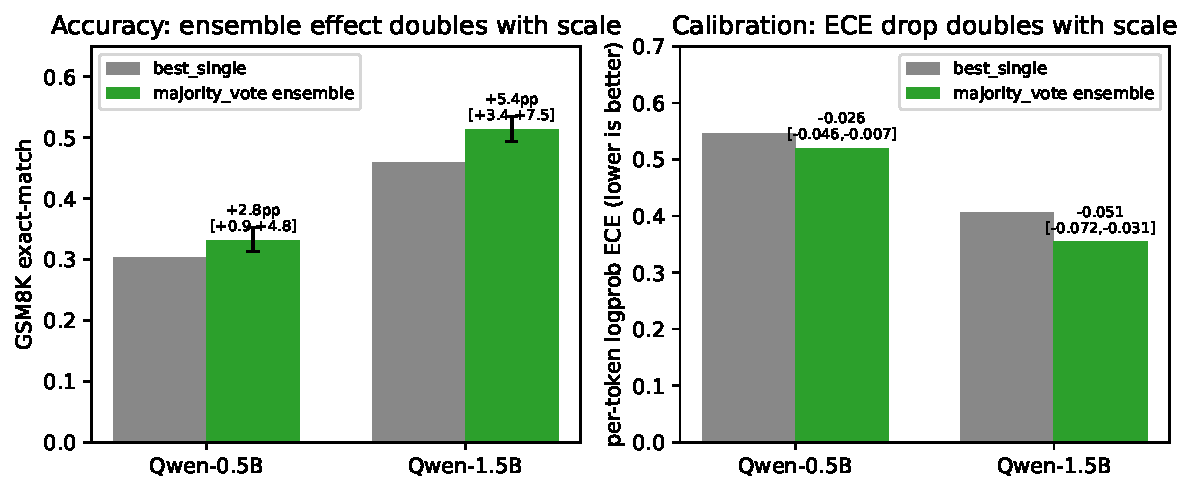
\includegraphics[width=\columnwidth]{figures/fig_gsm8k_scale_doubling.pdf}
\caption{GSM8K decoder scaling on cells with a known selection defect. \texttt{best\_single} here was selected on the same test split it is evaluated on (L12(i)), so these differences support no positive ensembling claim; whether the benchmark is also contaminated is open (L12(ii)). The embedded panel titles are from an earlier framing and should be read as descriptive, not as a result.}
\label{fig:gsm8k_scale}
\end{figure}

\section{Distillation $\alpha\times T$ sweep (Qwen-0.5B MNLI)}\label{app:distill}
We sweep the soft-target distillation HPs $\alpha\in\{0.5,0.7,0.9\}$ (weight on soft-target loss vs.\ hard-target) and $T\in\{1,2,4,8\}$ (softmax temperature on teacher logits) for a $4\times4$ grid on Pool-A Qwen-0.5B MNLI. Vanilla single (no distillation): $0.8365 / 0.0465$ (acc/ECE). Soft-vote ensemble target: $0.8495 / 0.0187$. Best student: $(\alpha{=}0.9, T{=}4)$ yields $0.8479 / 0.0397$, recovering $87\%$ of the soft-vote accuracy gain at $1\times$ student cost. Across the grid, accuracy varies $\pm0.003$ and ECE varies $\pm0.012$; the sweep is locally robust. The same sweep on Pool-A BERT-base MNLI yields a student strictly worse than vanilla single on both arms, consistent with the encoder-accuracy-REVERSED finding (no signal to distill).

\section{Frontier regression features}\label{app:features}
For each (pool, method, baseline) cell we extract a feature vector $\phi\in\mathbb{R}^{d}$ used to fit the diversity-quality frontier. Features are grouped:
\begin{itemize}[leftmargin=*]
\item \textbf{prediction\_space} ($d{=}3$): pairwise prediction disagreement (mean over pool pairs), logit correlation (mean over pool pairs), error overlap (Jaccard on incorrect examples).
\item \textbf{parameter\_space} ($d{=}3$): mean weight cosine distance, mean centered-kernel-alignment (CKA) on penultimate layer, weight $L_2$ norm spread.
\item \textbf{HP entropy} ($d{=}2$): entropy of $r$-distribution within pool, entropy of $\{lr, \alpha\}$ joint distribution.
\item \textbf{ensemble quality} ($d{=}2$): pool mean val\_acc, pool best-single val\_acc.
\end{itemize}
Per-feature ablation on the encoder \texttt{acc vs n\_rank} slice: dropping the prediction\_space group crashes $R^2$ from $+0.62$ to $-24.5$ ($\Delta R^2 {=}{+}25.0$); dropping parameter\_space drops $R^2$ by $0.56$; dropping HP-entropy \emph{improves} $R^2$ by $0.08$ (HP entropy adds in-sample fit but no out-of-pool signal). A single-group ``only prediction\_space'' model achieves $R^2{=}0.634$, \emph{higher} than the full feature set.

\section{Cell adjudication pseudocode}\label{app:pseudocode}
{\footnotesize\begin{verbatim}
def adjudicate(pool, method, baseline,
               metric, B=5000):
  # Per-example predictions on test split
  ens  = load_predictions(pool, method)
  base = load_predictions(pool, baseline)
  gold = load_labels()
  # Per-example metric residual
  if metric == 'acc':
    d = (ens == gold) - (base == gold)
  elif metric == 'ece':
    d = ece_bin_residual(ens, gold) \
      - ece_bin_residual(base, gold)
  N = len(d)
  # Paired bootstrap CI
  boot = []
  for _ in range(B):
    idx = np.random.randint(0, N, N)
    boot.append(d[idx].mean())
  delta = float(np.mean(boot))
  ci_lo = float(np.percentile(boot, 2.5))
  ci_hi = float(np.percentile(boot, 97.5))
  # Sign-flip p-value
  obs = abs(d.mean())
  null_count = 0
  for _ in range(B):
    signs = np.random.choice([-1, 1], N)
    if abs((d * signs).mean()) >= obs:
      null_count += 1
  p = 2 * null_count / B
  # Adjudication
  if   ci_lo > 0: label = 'supported'
  elif ci_hi < 0: label = 'reversed'
  else:           label = 'unsupported'
  return {
    'delta': delta, 'ci': (ci_lo, ci_hi),
    'p_raw': p, 'adjudication': label,
    'N_test': N,
  }
\end{verbatim}}

\section{Cluster orchestration details}\label{app:cluster}
The 50-node RTX 3060 12GB cluster is orchestrated via \texttt{sweep\_runner.py}, an in-house SSH-based fan-out engine. Each sweep config (JSON) declares a Cartesian parameter grid; the runner stages source files, assigns one (param-combination, node) pair per slot, and tracks per-job exit codes in \texttt{sweep\_runs/<name>/results.json}. Pool-A sweeps complete in $\sim$4--8 GPU-hours wall clock (parallelism factor $\sim$20); Pool-B/C in $\sim$16--24 hours. The v1.2 A6000 sweeps (Qwen-3B, Qwen-7B, Llama-3.1-8B-Instruct on GSM8K) use \texttt{local\_gpu\_runner.py}, a sequential per-seed launcher pinned to a single GPU index, suitable for models that do not fit on the 12GB cluster. Adapter weights are pulled back via \texttt{collect\_remote\_adapters.py} and assembled into pool manifests via \texttt{build\_adapter\_pool.py}; the manifest schema is documented in \texttt{scripts/validate\_pool.py}.

\section{Cost-savings analysis: derivation and stratified breakdown}\label{app:cost}

{\sloppy This appendix presents the cost-savings table (Table~\ref{tab:cost}) and stratifies by pool type and method. The corpus comparison uses $887$ compute-matched cells: (A)~\emph{blind} --- always use \texttt{soft\_vote} (the default in much prior PEFT-ensembling work); (B)~\emph{routed} --- per-cell oracle pick over the four methods (\texttt{soft\_vote}, \texttt{majority\_vote}, \texttt{logit\_avg}, \texttt{greedy\_soup}) approximating D1--D5. Inference cost is single-adapter forward-passes per query: $N$ (pool size) for vote-based methods, $1$ for \texttt{greedy\_soup} (outputs a single merged checkpoint).\par}

\begin{table}[h]
\centering
\caption{Cost of blind ensembling. Mean signed $\Delta$ (positive$=$ensemble better), \%~cells REVERSED, median inference cost (adapter-passes/query). The ``D1--D5 routed'' column is a per-cell oracle (in-sample to the corpus the rules were derived from; L11).}
\label{tab:cost}
\small
\setlength{\tabcolsep}{3pt}
\begin{tabular}{@{}lrrrrrr@{}}
\toprule
 & \multicolumn{3}{c}{Blind soft\_vote} & \multicolumn{3}{c}{D1--D5 routed} \\
\cmidrule(lr){2-4}\cmidrule(lr){5-7}
Slice ($n$) & $\overline{\Delta}$ & REV & cost & $\overline{\Delta}$ & REV & cost \\
\midrule
Enc acc (54)   & $-3.8$pp & $31\%$ & $20{\times}$ & $+0.5$pp & $4\%$ & $\mathbf{1{\times}}$ \\
Dec acc (50)   & $+0.6$pp & $0\%$  & $18{\times}$ & $+0.8$pp & $0\%$ & $15{\times}$ \\
Enc ECE (63)   & $+2.4$pp & $10\%$ & $20{\times}$ & $+3.6$pp & $2\%$ & $20{\times}$ \\
Dec ECE (50)   & $+3.5$pp & $0\%$  & $18{\times}$ & $+3.5$pp & $0\%$ & $18{\times}$ \\
\midrule
All (217)      & $+0.7$pp & $11\%$ & $19{\times}$ & $+2.1$pp & $2\%$ & $17{\times}$ \\
\bottomrule
\end{tabular}
\end{table}

\paragraph{Oracle method distribution.} The per-cell argmax (Table~\ref{tab:cost}, ``D1--D5 routed'') picks: \texttt{greedy\_soup} on $45/104$ accuracy groups ($33/54$ encoder, $12/50$ decoder) --- consistent with D1's preference for soup-merge on encoders; \texttt{soft\_vote} on $19/104$ accuracy and $88/113$ ECE groups --- consistent with D1+D3; \texttt{majority\_vote} on $23/104$ accuracy (predominantly decoder GSM8K, D3); \texttt{logit\_avg} on $17/104$ accuracy and $12/113$ ECE.

\paragraph{Deployable D1--D5 rule.} A deployable rule using only \emph{family} (encoder/decoder), \emph{convergence} (fraction of pool above chance), \emph{metric} (accuracy vs.\ ECE), and \emph{output space} (classification vs.\ generation) recovers most of the oracle gain in our cells; feature importances align with App.~\ref{app:features}. The remaining gap to per-cell oracle is the cost of not running \texttt{compute\_match.py} per-cell against the released $1{,}028$-cell baseline.

\end{document}
